\documentclass[a4paper]{report}
\usepackage{amsmath,amssymb,booktabs,bm,caption,enumerate,float,geometry,graphicx,indentfirst,multirow,setspace,titlesec}
\geometry{left=4.5cm,right=4.5cm,top=4cm,bottom=4cm}
\captionsetup[figure]{labelsep=period}
\captionsetup[table]{labelsep=period}
\begin{document}
	\renewcommand\thesection{\arabic{section}}
	\begin{Large}
		\begin{center}
			\setlength{\baselineskip}{14pt}
			\vspace{1.25cm}
			\rule[0cm]{11.2cm}{0.03em}\\
			\vspace{0.5cm}
			\textsc{UM-SJTU Joint Institute}\\
			\vspace{0.25cm}
			\textsc{Physics Laboratory\\(Vp141)}
			\vspace{0.3cm}
			\rule[0cm]{11.8cm}{0.05em}
			\vspace{4.9cm}\\
			\textsc{Laboratory Report}
		\end{center}
	\end{Large}
	\vspace{0.85cm}
	\begin{large}
		\begin{center}
			\textsc{Exercise 3}
			\vspace{1em}\\
			\textsc{Simple Harmonic Motion:\\Oscillations in Mechanical Systems}
		\end{center}
		\vspace{6cm}
	\end{large}
	\begin{tabular}{l l l}
	Name: Yihua Liu&ID:518021910998&Group 9\\
	Name: Guanghan Xi&ID: 518021910778&Group 9\\
	&&\\
	Date: \today&&\\
	\end{tabular}
	\thispagestyle{empty}
	\newpage
	\section{Introduction}
	The main objective of this experiment is to study simple harmonic oscillations. We will learn how to calculate the spring constant and effective mass for two springs and the way to use the air track. We will explore the relationship between the period of the oscillation and the mass of the oscillator, the relationship between the oscillation period and its amplitude, and the relationship between its maximum speed and the amplitude.
	
	The simple harmonic motion is the simplest periodic motion. The position of the oscillator is a sine or cosine function on time. Within the elastic limit of deformation, the relationship between the force $F_x$ and the distance stretched or compressed $x$ is described by Hooke's Law
	\begin{equation}
	F_x=kx
	\end{equation}
	where $k$ is the spring constant, examining the elasticity of a spring. In this experiment, we use the Jolly balance as the measurement device to find the spring constant. The force $F_x$ is called the restoring force because the force tries to restore the spring back to the equilibrium, different from the elastic force in an opposite direction.
	\begin{figure}[H]
		\centering
		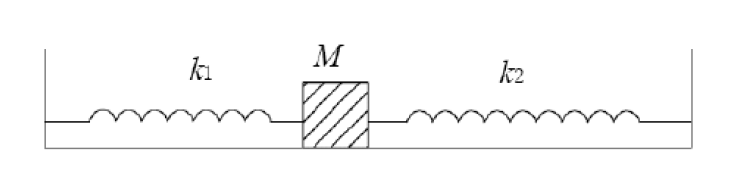
\includegraphics[width=0.5\linewidth]{1.png}
		\caption{Mass-spring system.}
	\end{figure}
	As is shown in Figure 1, the block with mass $M$ on the air track are attached to both two ends by two springs. Using the air track can eliminate the friction between the underside surface of the block and the ground. Initially, the block is set at equilirium where we note the position coordinate $x=0$. We will measure both the spring constants $k_1$ and $k_2$ of the two springs. Ignoring damping and the mass of the springs, by Newton's second law of dynamics, the motion of the block can be expressed by the equation
	\begin{equation}
	M\dfrac{\mathrm{d}^2x}{\mathrm{d}t^2}+(k_1+k_2)x=0
	\end{equation}
	Solving Eq. (2), we have
	\begin{equation}
	x(t)=A\cos(\omega t+\phi_0)
	\end{equation}
	where $\omega_0=\sqrt{(k_1+k_2)/M}$ is the natural angular frequency of the motions, A is its amplitude, and $\phi_0$ is the initial phase. Furthermore, the natural period of the oscillation is
	\begin{equation}
	T=\dfrac{2\pi}{\omega_0}=2\pi\sqrt{\dfrac{M}{k_1+k_2}}
	\end{equation}
	
	However,  when the mass of the springs cannot be neglected, we have to consider the effective mass. The effective mass of the oscillator is the sum of the effective mass of the spring and the mass of the object. Then, the angular frequency of the system becomes
	\begin{equation}
	\omega_0=\sqrt{\dfrac{k_1+k_2}{M+m_0}}
	\end{equation}
	where $m_0$ is the effective mass of the spring. It is just one third of the spring's actual mass.
	
	Then we study the mechanical energy in harmonic oscillations. The mechanical energy is composed of potential energy $U=kx^2/2$ and kinetic energy $K=mv^2/2$. By the conservation law of mechanical energy, the maximum kinetic energyy $K_{\rm{max}}$ is equal to the maximum potential energy $U_{\rm{max}}$ when the object is at the maximum displacement $x=0$ at equilibrium and $x=\pm A$ where $v=0$ respectively. Hence,
	\begin{equation}
	k=\dfrac{mv_{max}^2}{A^2}
	\end{equation}
	\section{Experimental setup}
	Generally, the measurement device includes springs, masses, electronic balance, electronic timer, air track, and Jolly balance. The Jolly balance consists of the following components from top to bottom: sliding bar with metric scale, vernier, small mirror with a horizontal middle line, fixed tube also with a horizontal middle line, know, and spring attached to the top of the sliding bar, shown in Figure 2.
	\begin{figure}[H]
		\centering
		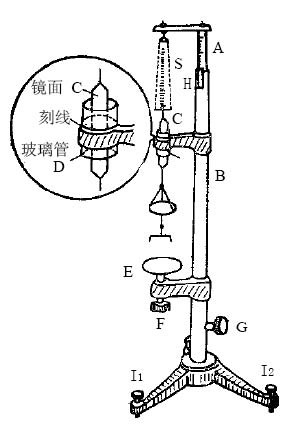
\includegraphics[width=0.5\linewidth]{2.jpg}
		\caption{Jolly balance.}
	\end{figure}
	To prepare for the measurement of the spring constant, we first need to place the small mirror in the fixed glass tube and coincide the line on the mirror, the line on the tube, and its reflection by adjusting the knob with no weiget on the bottom end of the spring. We record the scale reading $L_1$.
	
	Then, on the bottom end of the spring we add mass $m$ and adjust the knob to make the three lines coincide again and get the reading on scale as $L_2$. Hence, we can find the spring constant as
	\begin{equation}
	k=\dfrac{mg}{L_2-L_1}
	\end{equation}
	After measuring $L_2$ and $L_1$ for several times with different masses $m$, we can do a linear fit with the least squares method to find a better estimation of the spring constant.
	\begin{figure}[H]
		\centering
		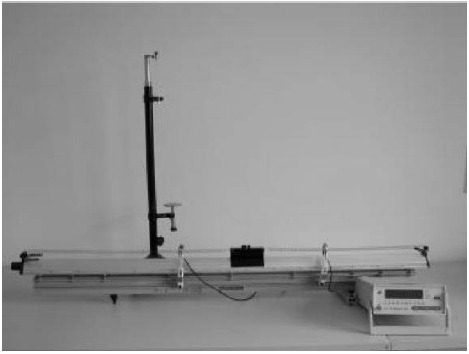
\includegraphics[width=0.9\linewidth]{3.jpg}
		\caption{The experimental setup.}
	\end{figure}
	For the photoelectric measuring system shown in Figure 3, there are two parts: an electronic timer and two photoelectric gates. The shutter can be placed to cover the light emitted from the top so that the electronic timer can receive a signal.
	\begin{figure}[H]
		\centering
		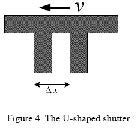
\includegraphics[width=0.5\linewidth]{4.jpg}
		\caption{The U-shape sutter.}
	\end{figure}
	When measuring the period, we use I-shaped shutters. However, for speed measurements, we use U-shape shutters that the signals are sent twice for every pass through, which is shown in Figure 4. We can read the time interval $\Delta t$ from the recording on the timer and the distannce $\Delta x=\frac{1}{2}(x_{in}+x_{out})$ between two signals. Hence, we can calculate the speed of the object when passing through the gate as $v=\Delta x/\Delta t$.
	
	The appratus is listed in Table 1, including measuring instruments together with their parameters.
	\begin{table}[H]
		\centering
		\begin{tabular}{cccc}
			\hline
			Instruments&Quantity Measured&Range&Precision\\
			\hline
			Electronic Scale&Mass&6000 [g]&$\pm$ 0.01 [g]\\
			Metric Scale on the Air Track&Amplitude&N/A&$\pm$ 0.01 [cm]\\
			Electronic Timer&Time interval&N/A&$\pm$0.0001[s] (T)\&$\pm$0.00001[s]($S_2$)\\
			Caliper&$x_in$ and $x_out$&150 [mm]&$\pm$ 0.02 [mm]\\
			\hline
		\end{tabular}
	\caption{Experimental setup.}
	\end{table}
	\section{Measurement}
	\subsection{Spring Constant}
	We first set the Jolly balance to be vertical and attach the spring as is shown in the experimental setup. Then we add a 20 g preload and adjust the knob $I_1$ and $I_2$ so that the mirror can move freely. Then check if the balance is parallel to the spring. If not, adjust knobs from. During the adjustment, we look at the Jolly balance from two orthogonal directions to make sure that the balance coincides with the spring.
	
	Then, we adjust knob on the bottom G to coincide the three lines in the tube, set and record the initial position $L_0$ within 5.0 ~ 10.0 cm on the scale. Next, we add mass $m_1$ and record another position $L_1$.
	
	After that, we keep adding masses and measuring the positions for six times and record the corresponding order of the six masses. After recording, we calculate the spring constant $k_1$ by the least squares method.
	
	Then, we replace spring 1 with spring 2 and repeat the steps above to calculate $k_2$. After that, we take down the preload and repeat the steps above for the series of spring 1 and spring 2 to calculate $k_3$. Finally, we compare the experimental value with the theoretical value.
	\subsection{Relation Between the Oscillation Period $\bm{T}$ and the Mass of the Oscillator $\bm{M}$}
	(a) Adjust the air track so that it is horizontal.
	
	First,we adjust the air track to be horizontal without anything on before turning on the air pump to protect the air track. After we turn on the air pump, we check whether there are any holes on the air track blocked. If there are any blocked holes, we would call the instructor.
	
	Then, we place the cart on the air track still and adjust the single knob on it until the object can moves freely back and forth in both directions.
	
	(b) Horizontal air track
	
	In a horizontal air track, we attach the two springs to both sides of the cart and set the I-shape shutter on it with the photoelectric gate at the equilibrium position.
	
	First we add mass $m_1$ and release the cart in one direction and it oscillates about the photoelectric gate. The releasing position is about 5 cm. We relaase the cart with a caliper. Then, we set the timer to the "T" mode that the timer will record the time of ten oscillation periods automatically and record the period and the mass of the oscillator.
	
	Then, we add masses to the object and repeat releasing the cart and recording the measurements for 5 times. After recirdubg, we analyze the relationship between the period $T$ and the mass $M$ from the graph.
	
	(c)Inclined air track
	
	To control the inclination of the air track, we place every three of the plastic plates under the air track increased each time. We repeat doing measurements in (b) for tww different inclinations with 3 and 6 plastic plates laid. After recording, we analyze the relationship between the period $T$ and the mass $M$ from the graph.
	\subsection{Relation Between the Oscillation Period $\bm{T}$ and the Amplitude $\bm{A}$}
	We first keep original number of masses on the cart and change the amplitude for six times, such as 5.0/10.0/15.0/.../30.0 cm. We can then apply linear fit to the measurements and discuss the relationship between the amplitude $A$ and the period $T$ with correlation coefficient $\gamma$.
	\subsection{Relaiton Between the Maximum Speed and the Amplitude}
	We first measure the outer and inner distance of the U-shape shutter as $x_{\rm{out}}$ and $x_{\rm{in}}$ respectively by a caliper. We can get the distance $\Delta x=(x_{\rm{out}}+x_{\rm{in}})/2$. Then we use U-shape instead of I-shape shutter. We set the timer into the mode "$S_2$" and oscillate the cart. After that, we record the readings of the time interval $\Delta t$ when the two subsequent readings have the same digits to the left of the decimal point.
	
	We change the amplitude for six times again like about 5.0/10.0/15.0/.../30.0 cm. Finally, we can obtain the maximum speed $v_{max}$ for different amplitude $A$ and then the spring constant. We can compare the spring constant $k$ to that of the first part of the experiment.
	\subsection{Mass measurement}
	First we adjust the elctronic balance whenever we use it so that the level bubble is in the circular center. Then, we gradually add masses according to the previously recorded order. After that, we measure the cart with the U-shape and the I-shape shutter respectively and the mass of spring 1 and spring 2. Finally, we record the measurements after the display on the scale vanishes.
	\section{Results and Calculations}
	\subsection{Spring Constant}
	In this experiment, we measure $L$ for spring 1, spring 2, and their series. The results are shown in Table 2.
	\begin{table}[H]
		\centering
		\begin{tabular}{|c|c||c|c||c|c|}
			\hline
			\multicolumn{2}{|c||}{spring 1 [cm] $\pm$ 0.01 [cm]}&\multicolumn{2}{|c||}{spring 2 [cm] $\pm$ 0.01 [cm]}&\multicolumn{2}{|c|}{series [cm] $\pm$ 0.01 [cm]}\\
			\hline
			$L_0$&5.21&$L_0$&3.13&$L_0$&5.80\\
			\hline
			$L_1$&7.28&$L_1$&5.04&$L_1$&9.68\\
			\hline
			$L_2$&9.31&$L_2$&6.93&$L_2$&13.51\\
			\hline
			$L_3$&11.18&$L_3$&8.97&$L_3$&17.55\\
			\hline
			$L_4$&13.20&$L_4$&10.90&$L_4$&21.51\\
			\hline
			$L_5$&15.14&$L_5$&12.73&$L_5$&25.51\\
			\hline
			$L_6$&17.25&$L_6$&14.81&$L_6$&29.46\\
			\hline
		\end{tabular}
		\caption{Spring constant measurment data.}
	\end{table}
	Besides, we measure the weight added and the results are shown in Table 3.
	\begin{table}[H]
		\centering
		\begin{tabular}{|c|c|}
			\hline
			\multicolumn{2}{|c|}{$m$ [g] $\pm$ 0.01 [g]}\\
			\hline
			1&4.72\\
			\hline
			2&9.49\\
			\hline
			3&14.19\\
			\hline
			4&18.84\\
			\hline
			5&23.68\\
			\hline
			6&28.44\\
			\hline
		\end{tabular}
	\caption{Weight measurement data.}
	\end{table}
	We take the gravitational acceleration $g$ as 9.794 $\rm{m/s^2}$, we can derive the $\Delta l$ and $mg$ for spring 1 in Table 4.
	\begin{table}[H]
		\centering
		\begin{tabular}{|c|c|c|}
			\hline
			Measurement&$\Delta l$ [m] $\pm$ 0.00014 [m]&mg [N] $\pm$ 0.0001 [N]\\
			\hline
			1&0.0207&0.0462\\
			\hline
			2&0.0410&0.0929\\
			\hline
			3&0.0597&0.1390\\
			\hline
			4&0.0799&0.1845\\
			\hline
			5&0.0993&0.2319\\
			\hline
			6&0.1204&0.2785\\
			\hline
		\end{tabular}
	\caption{$\Delta l$ and $mg$ for spring 1.}
	\end{table}
	We can plot a graph of linear fit for $mg$ vs. $\Delta l$.
	\begin{figure}[H]
		\centering
		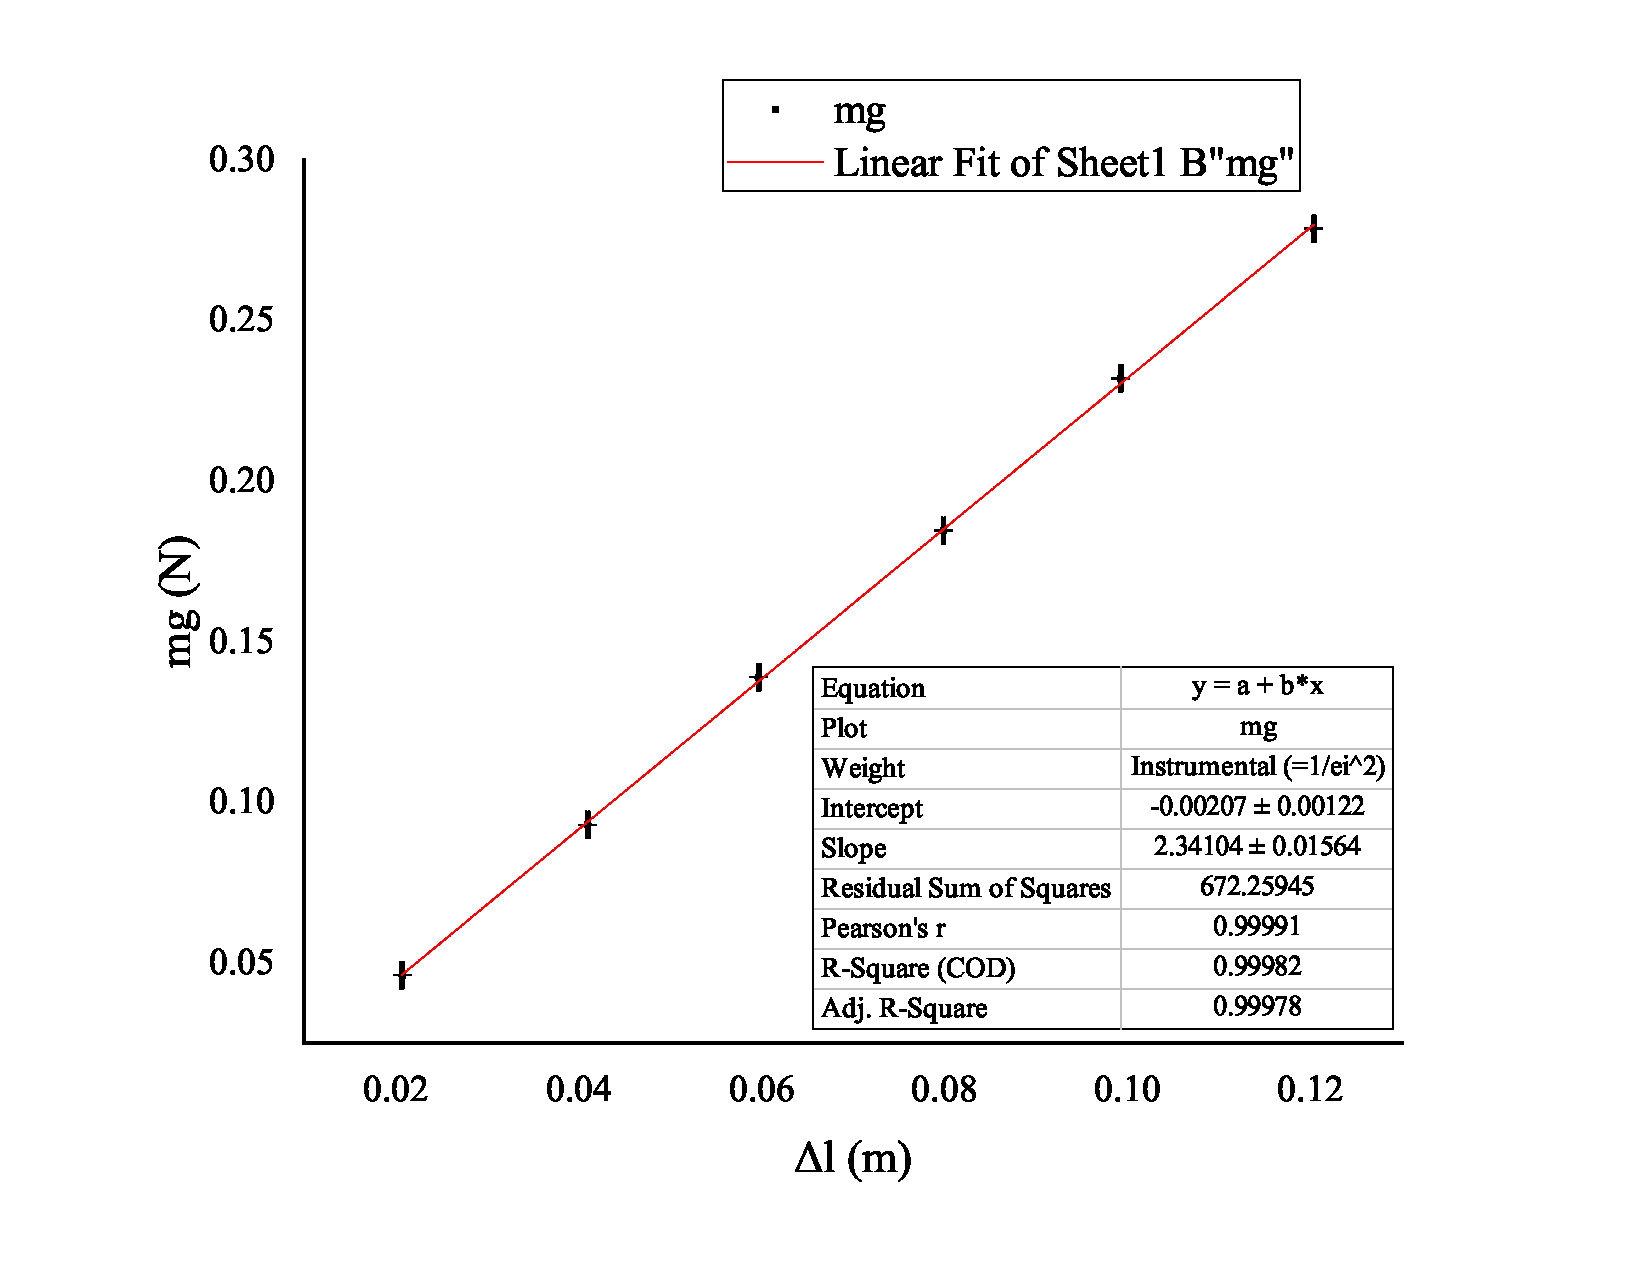
\includegraphics[width=1\linewidth]{5.eps}
		\caption{$mg$ v.s. $\Delta l$ for spring 1.}
	\end{figure}
	The value of the spring constant can be found from the graph $mg$ vs. $\Delta l$ in Figure 5. From a linear fit to $mg=\alpha\Delta l+\beta$ we have the slope $\alpha=2.34104$ N/m and the intercept $\beta=-0.00207$ N with standard errors $u_{\alpha}=0.01564$ N/m and $u_{\beta}=0.00122$ N and $R^2=0.99982$. By Eq. (7), the spring constant
	\begin{equation*}
	k_1=\alpha=(2.34\pm0.04)\rm{N/m}
	\end{equation*}
	with the uncertainty equal to the CI Half-Width
	\begin{equation*}
	u_{k_1}=0.04\ \rm{N/m}
	\end{equation*}
	and relative uncertainty 1.7\%.
	Analogously, for spring 2,
	\begin{table}[H]
		\centering
		\begin{tabular}{|c|c|c|}
			\hline
			Measurement&$\Delta l$ [m] $\pm$ 0.00014 [m]&mg [N] $\pm$ 0.0001 [N]\\
			\hline
			1&0.0191&0.0462\\
			\hline
			2&0.0380&0.0929\\
			\hline
			3&0.0584&0.1390\\
			\hline
			4&0.0777&0.1845\\
			\hline
			5&0.0960&0.2319\\
			\hline
			6&0.1168&0.2785\\
			\hline
		\end{tabular}
	\caption{$\Delta l$ and $mg$ for spring 2.}
	\end{table}
	We can plot a graph of linear fit for $mg$ vs. $\Delta l$.
	\begin{figure}[H]
		\centering
		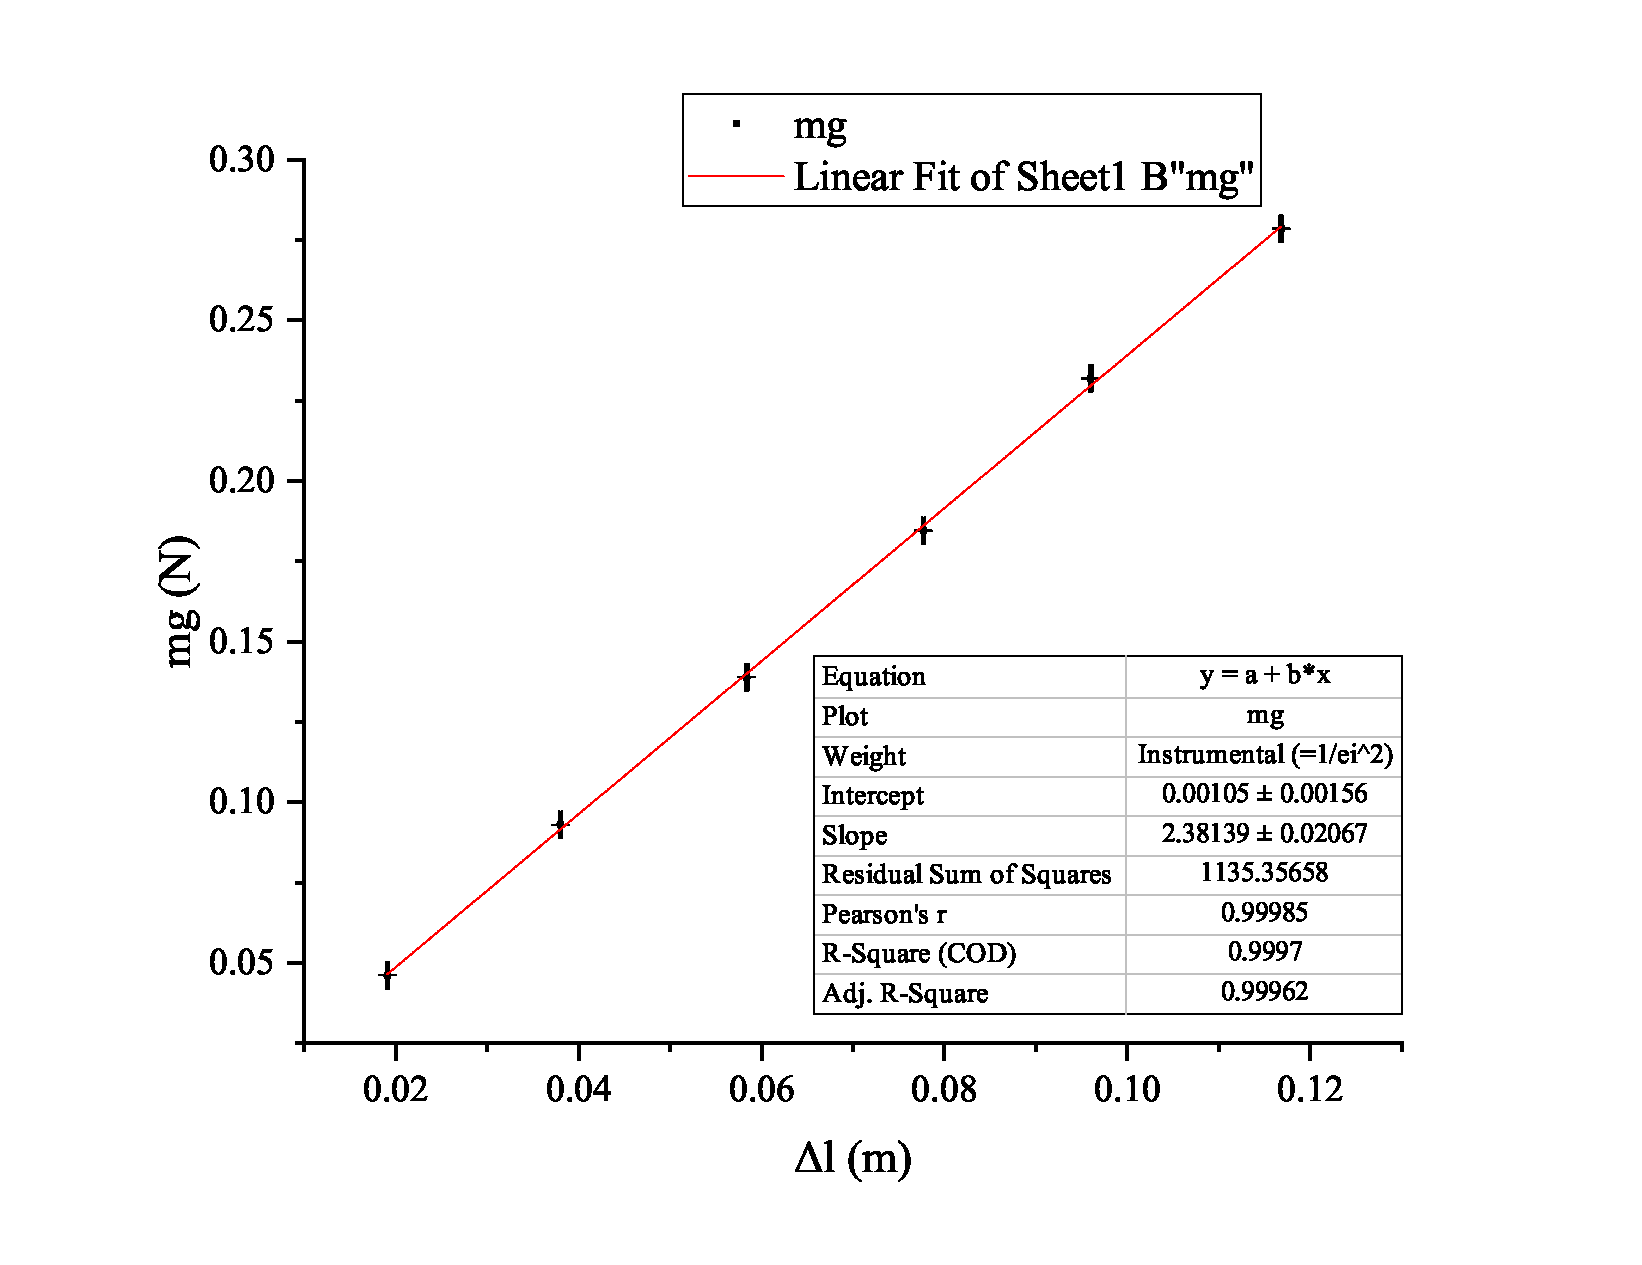
\includegraphics[width=1\linewidth]{6.eps}
		\caption{$mg$ v.s. $\Delta l$ for spring 2.}
	\end{figure}
	The value of the spring constant can be found from the graph $mg$ vs. $\Delta l$ in Figure 6. From a linear fit to $mg=\alpha\Delta l+\beta$ we have the slope $\alpha=2.38139$ N/m and the intercept $\beta=0.00105$ N with standard errors $u_{\alpha}=0.02067$ N/m and $u_{\beta}=0.00156$ N and $R^2=0.9997$. By Eq. (7), the spring constant
	\begin{equation*}
	k_2=\alpha=(2.38\pm0.06)\rm{N/m}
	\end{equation*}
	with the uncertainty equal to the CI Half-Width
	\begin{equation*}
	u_{k_2}=0.06\ \rm{N/m}
	\end{equation*}
	and relative uncertainty 3\%.
	Analogously, for the series of spring 1 and spring 2,
	\begin{table}[H]
		\centering
		\begin{tabular}{|c|c|c|}
			\hline
			Measurement&$\Delta l$ [m] $\pm$ 0.00014 [m]&mg [N] $\pm$ 0.0001 [N]\\
			\hline
			1&0.0388&0.0462\\
			\hline
			2&0.0771&0.0929\\
			\hline
			3&0.1175&0.1390\\
			\hline
			4&0.1571&0.1845\\
			\hline
			5&0.1971&0.2319\\
			\hline
			6&0.2366&0.2785\\
			\hline
		\end{tabular}
		\caption{$\Delta l$ and $mg$ for series.}
	\end{table}
	We can plot a graph of linear fit for $mg$ vs. $\Delta l$.
	\begin{figure}[H]
		\centering
		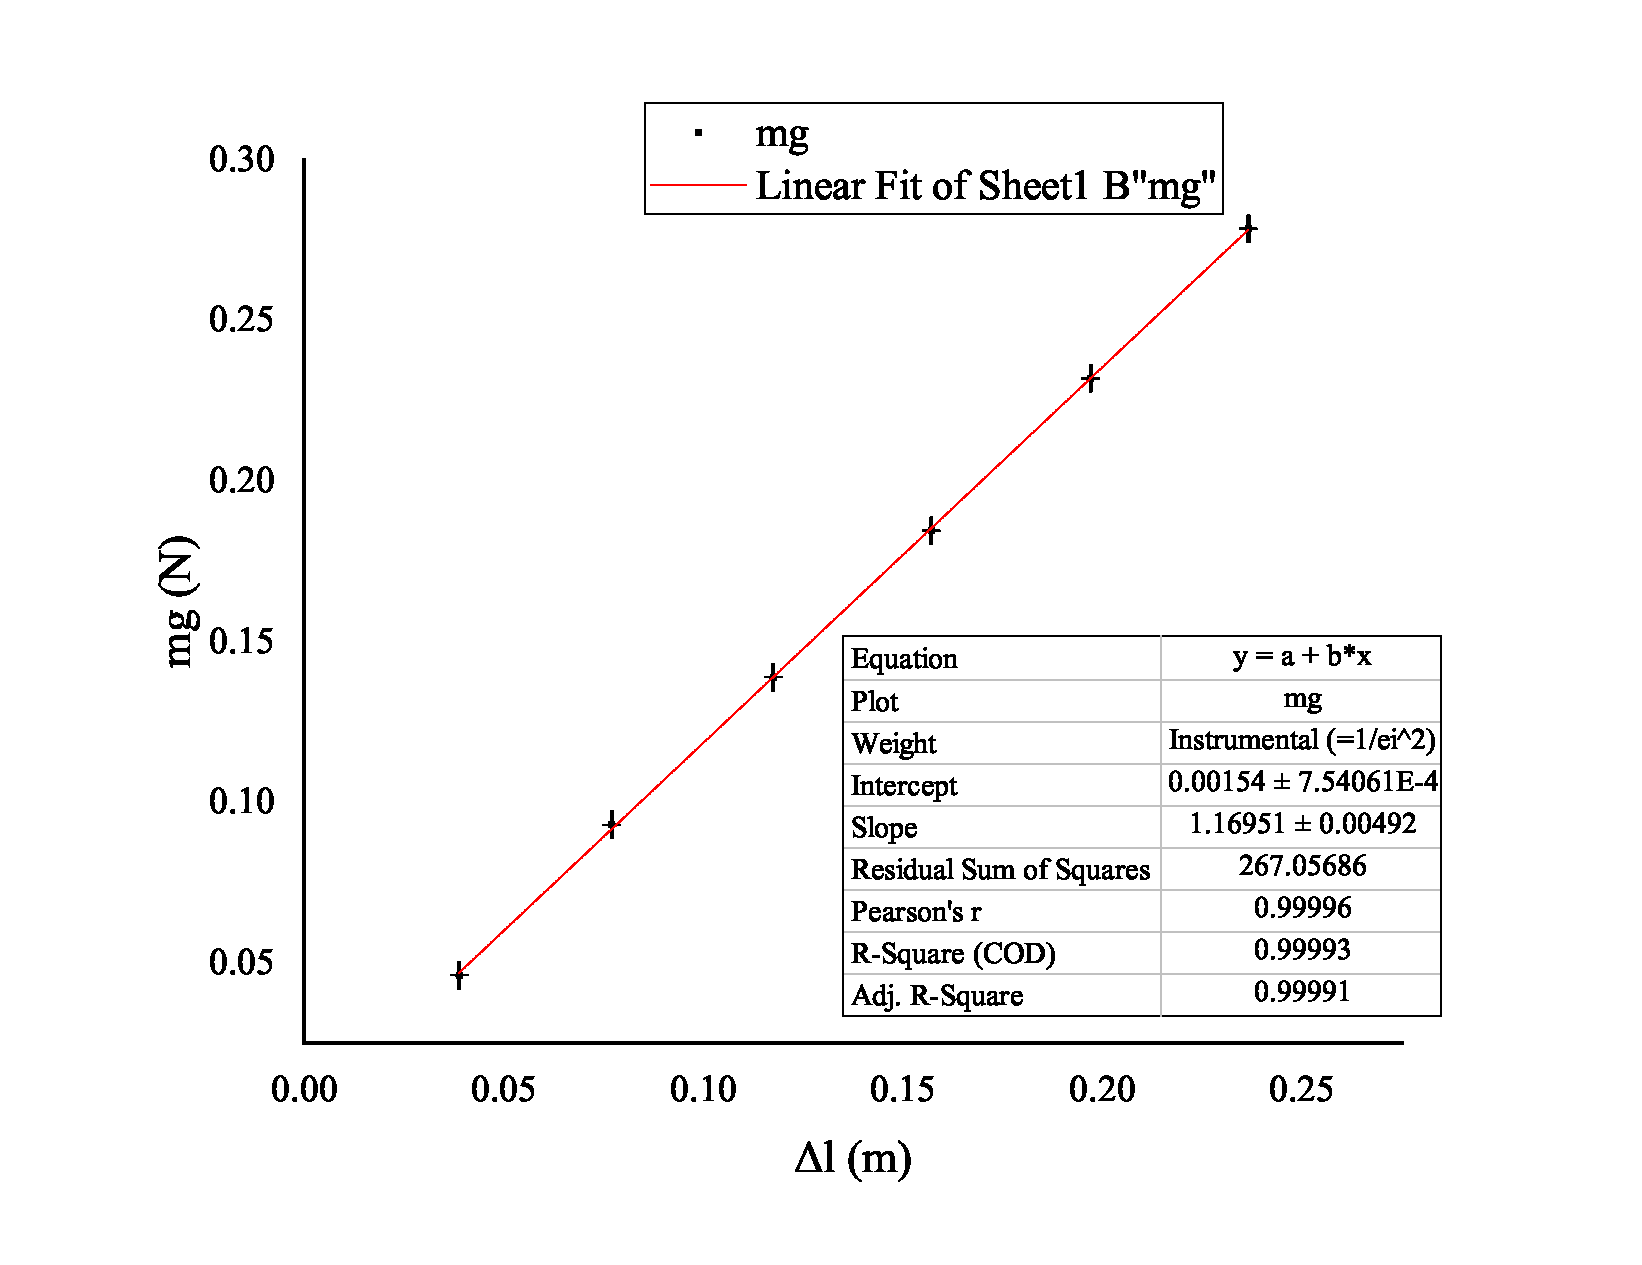
\includegraphics[width=1\linewidth]{7.eps}
		\caption{$mg$ v.s. $\Delta l$ for series.}
	\end{figure}
	The value of the spring constant can be found from the graph $mg$ vs. $\Delta l$ in Figure 6. From a linear fit to $mg=\alpha\Delta l+\beta$ we have the slope $\alpha=1.16951$ N/m and the intercept $\beta=0.00154$ N with standard errors $u_{\alpha}=0.00492$ N/m and $u_{\beta}=7.54061\times10^{-4}$ N and $R^2=0.99993$. By Eq. (7), the spring constant
	\begin{equation*}
	k_{1,2}=\alpha=(1.170\pm0.014)\rm{N/m}
	\end{equation*}
	with the uncertainty equal to the CI Half-Width
	\begin{equation*}
	u_{k_{1,2}}=0.014\ \rm{N/m}
	\end{equation*}
	and relative uncertainty 1.2\%.
	\subsection{Relation Between the Oscillation Period $\bm{T}$ and the Mass of the Oscillator $\bm{M}$}
	The data of measurements for the period and the mass is shown in Table 7.
	\begin{table}[H]
		\centering
		\begin{tabular}{|c|c||c|c||c|c|}
			\hline
			\multicolumn{6}{|c|}{ten periods [ms] $\pm$ 0.1 [ms]}\\
			\hline
			\multicolumn{2}{|c||}{horizontal}&\multicolumn{2}{|c||}{incline 1}&\multicolumn{2}{|c|}{incline 2}\\
			\hline
			$m_1$&12442.2&$m_1$&12447.4&$m_1$&12455.9\\
			\hline
			$m_2$&12602.0&$m_2$&12611.7&$m_2$&12610.2\\
			\hline
			$m_3$&12754.3&$m_3$&12760.3&$m_3$&12766.6\\
			\hline
			$m_4$&12913.8&$m_4$&12913.6&$m_4$&12923.3\\
			\hline
			$m_5$&13065.6&$m_5$&13072.6&$m_5$&13075.7\\
			\hline
			$m_6$&13224.6&$m_6$&13227.7&$m_6$&13231.9\\
			\hline
		\end{tabular}
	\caption{Measurement data for the $T$ vs. $M$ relation.}
	\end{table}
	The mass of the oscillator $M$ is equal to the equivalent mass of I-shape shutter plus the mass $m_i$. The equivalent mass $M_0=m_{\rm{obj}}+\frac{1}{3} m_{\rm{spr1\&2}}$. For I-shape it is 181.82 g = 0.18182 kg. Hence, we can calculate $T^2$ and $M$ and derive Table 8.
	\begin{table}[H]
		\centering
		\begin{tabular}{|c|c|c|c|c|}
			\hline
			\multirow{2}{*}{Measurement}&\multicolumn{3}{|c|}{$T^2$ [$\rm{s}^2$] $\pm$ 0.00003 [$\rm{s}^2$]}&\multirow{2}{*}{$M$ [kg] $\pm$ 0.00001 [kg]}\\
			\cline{2-4}
			&\multicolumn{1}{|c|}{Horizontal}&Incline 1&Incline 2&\\
			\hline
			1&1.54808&1.54938&1.55149&0.18654\\
			\hline
			2&1.58810&1.59055&1.59017&0.19131\\
			\hline
			3&1.62672&1.62825&1.62986&0.19601\\
			\hline
			4&1.66766&1.66761&1.67012&0.20066\\
			\hline
			5&1.70710&1.70893&1.70974&0.20550\\
			\hline
			6&1.74890&1.74972&1.75083&0.21026\\
			\hline
		\end{tabular}
	\caption{The relationship between the mass $M$ and the period's square $T^2$.}
	\end{table}
	Hence, we can do linear fit for $M$ vs. $T^2$ for three different inclinations. For the horizontal air track, the graph is Figure 8.
	\begin{figure}[H]
		\centering
		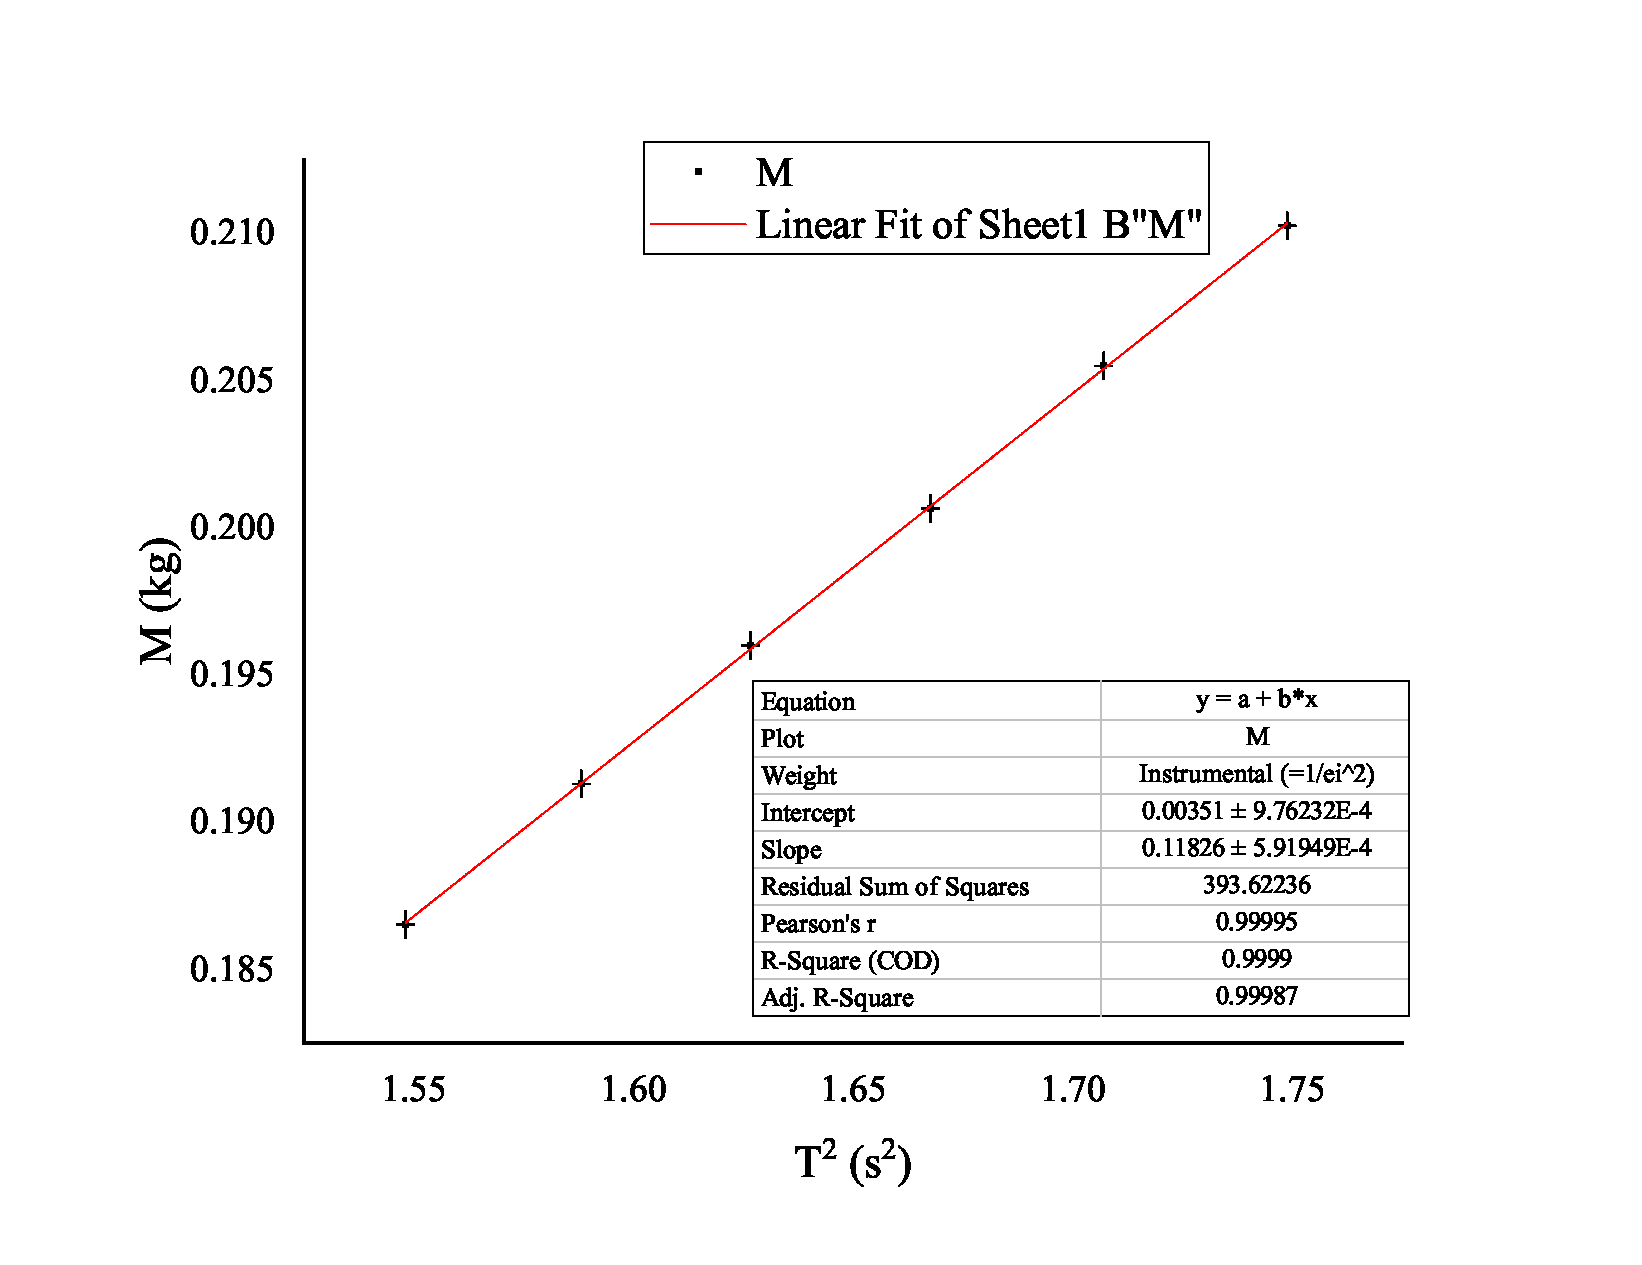
\includegraphics[width=1\linewidth]{8.eps}
		\caption{$M$ vs. $T^2$ for horizontal inlination.}
	\end{figure}
	Alternatively, the linear fit of $M$ vs. $T^2$ is given by equation $M=\alpha T^2+\beta$. From the graph we know that the slope $\alpha=0.11826\ \rm{kg/s^2}$, the intercept $\beta=0.00351$ kg, the uncertainty of the slope $u_{k_h}=0.002\ \rm{kg/s^2}$. The Pearson's r is equal to 0.99995 that is very close to 1, so $M$ and $T^2$ have a storng linear relationship.
	
	For Inclination 1, the graph is Figure 9.
	\begin{figure}[H]
		\centering
		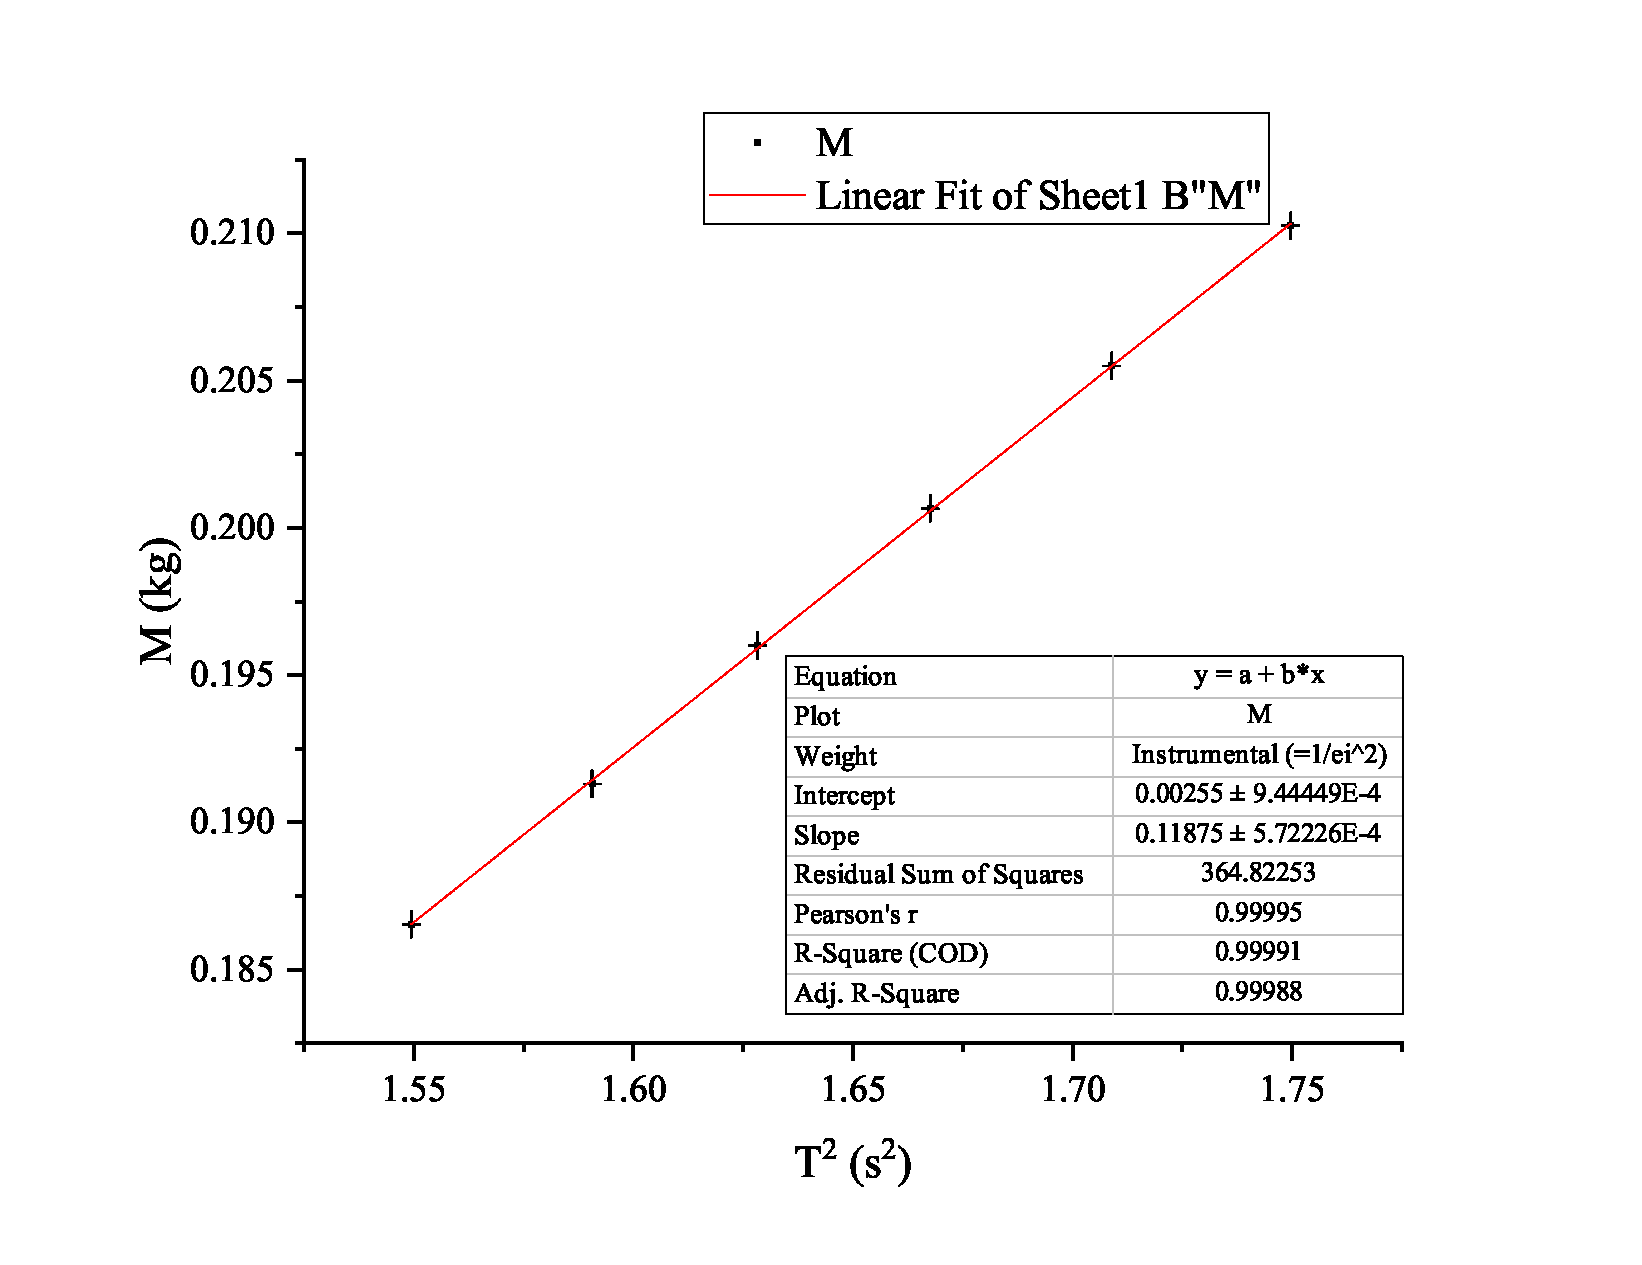
\includegraphics[width=1\linewidth]{9.eps}
		\caption{$M$ vs. $T^2$ for Inclination 1.}
	\end{figure}
	Alternatively, the linear fit of $M$ vs. $T^2$ is given by equation $M=\alpha T^2+\beta$. From the graph we know that the slope $\alpha=0.11875\ \rm{kg/s^2}$, the intercept $\beta=0.00255$ kg, the uncertainty of the slope $u_{k_{I1}}=0.002\ \rm{kg/s^2}$. The Pearson's r is equal to 0.99995 that is very close to 1, so $M$ and $T^2$ have a storng linear relationship.
	For Inclination 2, the graph is Figure 10.
	\begin{figure}[H]
		\centering
		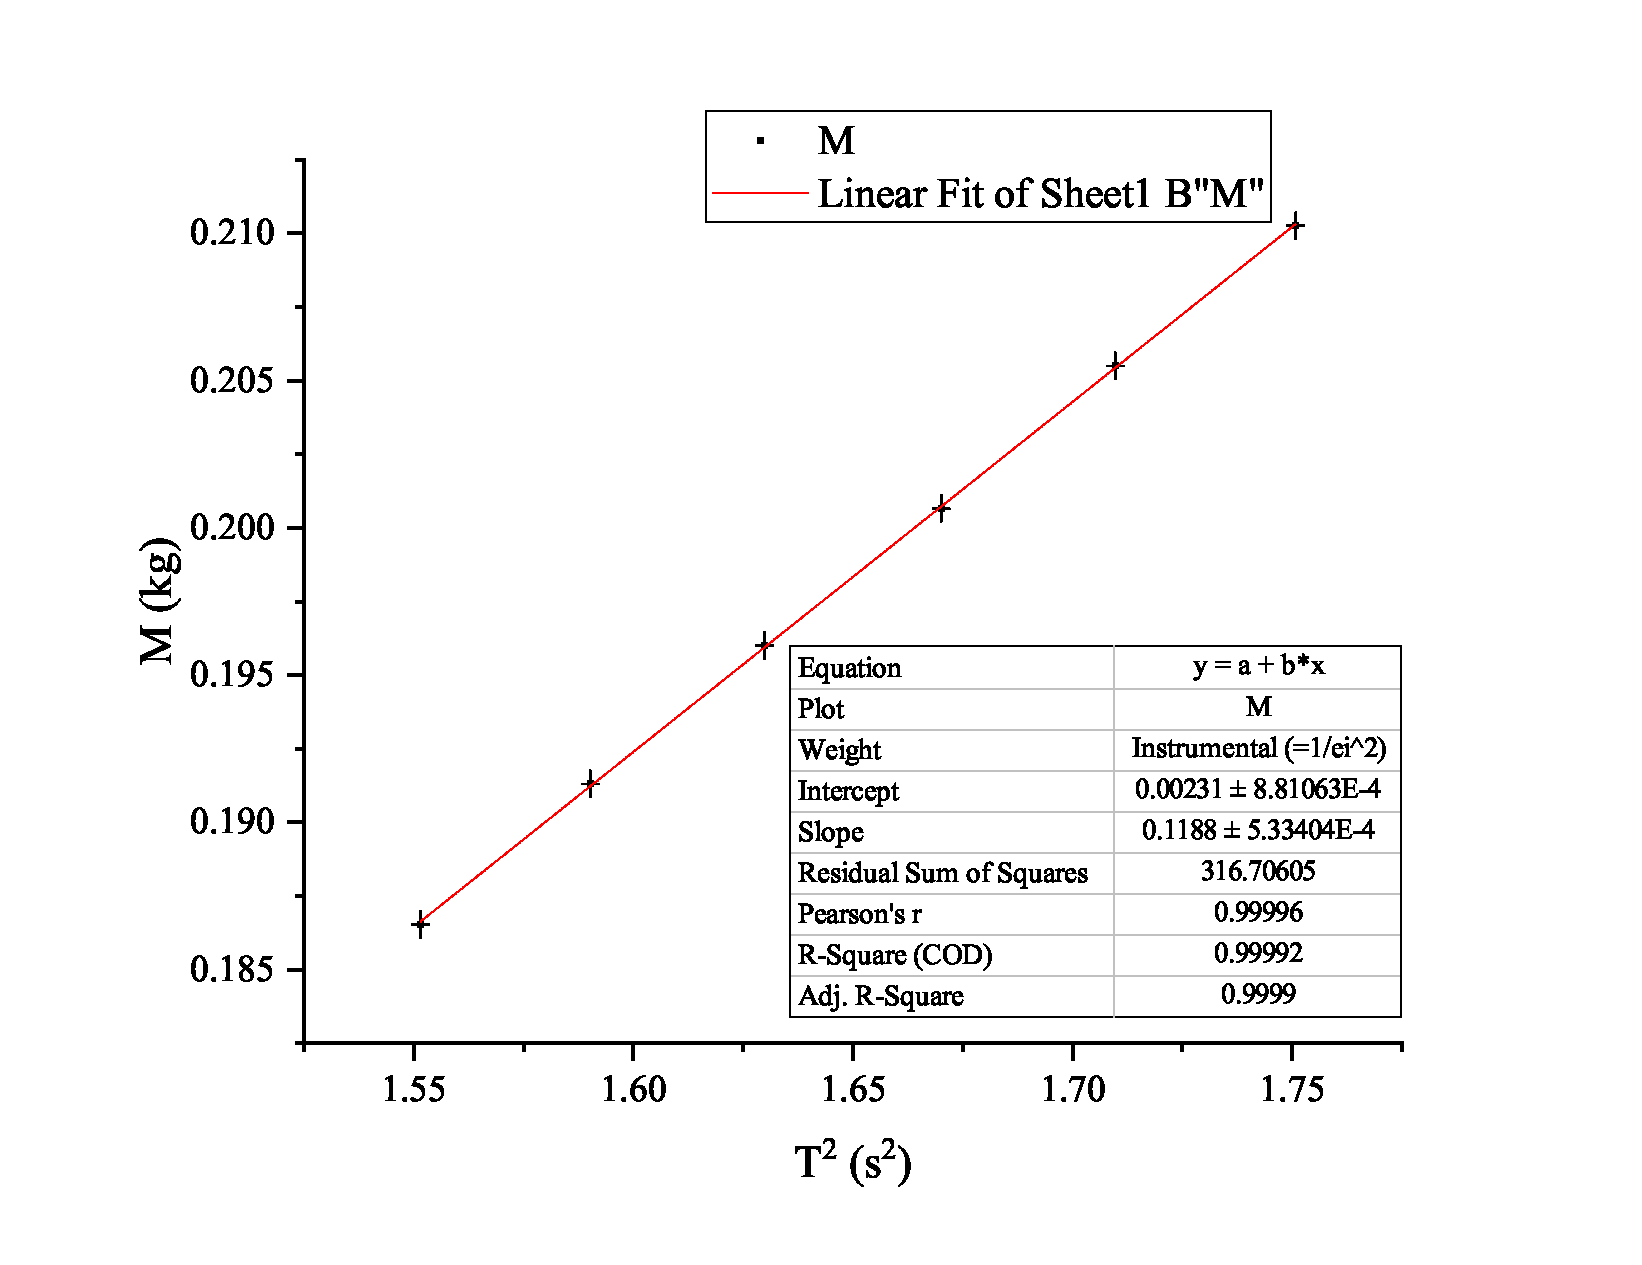
\includegraphics[width=1\linewidth]{10.eps}
		\caption{$M$ vs. $T^2$ for Inclination 2.}
	\end{figure}
	Alternatively, the linear fit of $M$ vs. $T^2$ is given by equation $M=\alpha T^2+\beta$. From the graph we know that the slope $\alpha=0.1188\ \rm{kg/s^2}$, the intercept $\beta=0.00231$ kg, the uncertainty of the slope $u_{k_{I2}}=0.001\ \rm{kg/s^2}$. The Pearson's r is equal to 0.99996 that is very close to 1, so $M$ and $T^2$ have a storng linear relationship.
	\subsection{Relation Between the Oscillation Period $\bm{T}$ and the Mass of the Oscillator $\bm{M}$}
	From Section 3.3 we have measurements data for the maximum speed and the amplitude shown in Table 9.
	\begin{table}[H]
		\centering
		\begin{tabular}{|c|c|c|}
			\hline
			\multicolumn{2}{|c|}{$A$ [cm] $\pm$ 0.1 [cm]}&ten periods [ms] $\pm$ 0.1 [ms]\\
			\hline
			1&5.0&12281.6\\
			\hline
			2&8.0&12285.8\\
			\hline
			3&11.0&12283.9\\
			\hline
			4&14.0&12285.9\\
			\hline
			5&17.0&12288.1\\
			\hline
			6&20.0&12288.3\\
			\hline
		\end{tabular}
	\caption{Data for the $T$ vs. $A$ relation.}
	\end{table}
	To study the relationship between $T$ and $A$, we still try to plot a linear fit as is shown in Figure 11.
	\begin{figure}[H]
		\centering
		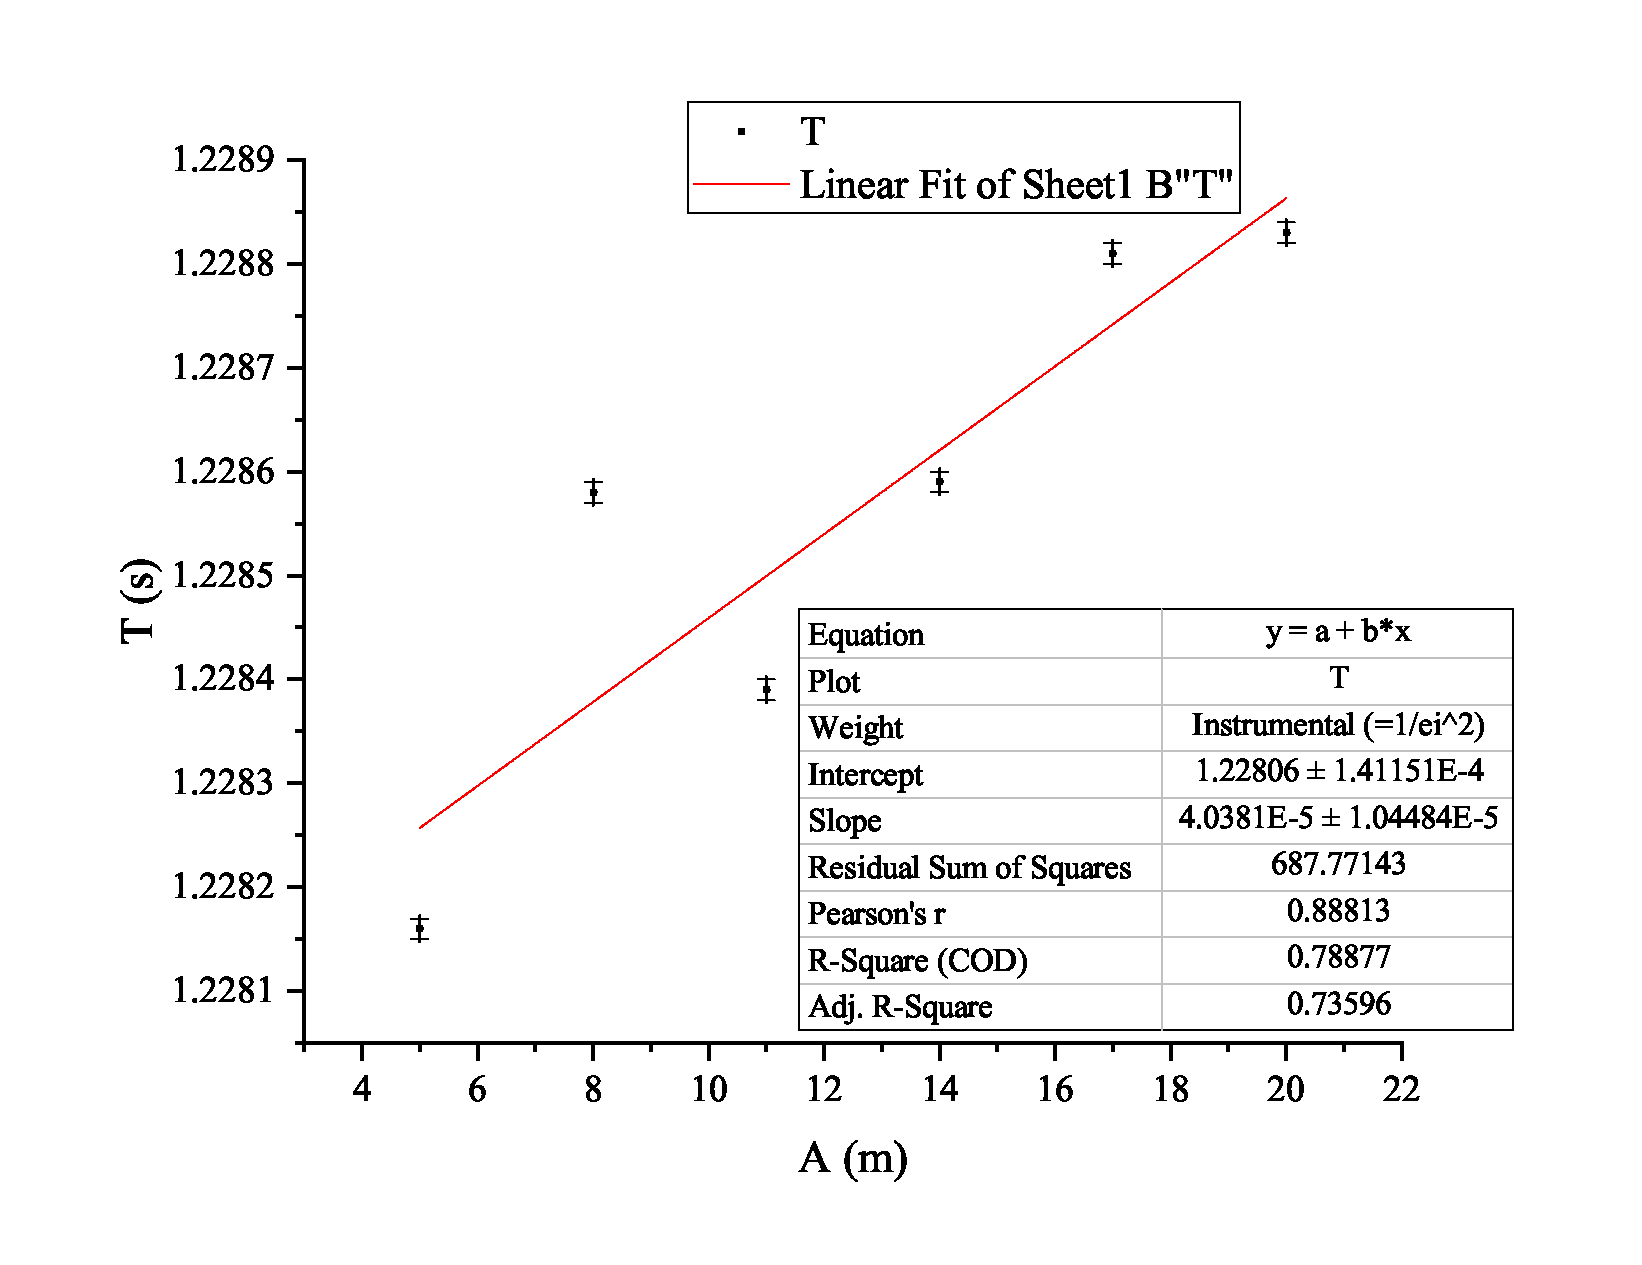
\includegraphics[width=1\linewidth]{11.eps}
		\caption{The Relationship between $T$ and $A$.}
	\end{figure}
	The linear fit of $M$ vs. $T$ is given by equation $M=\alpha T+\beta$. From the graph we know that the slope $\alpha=4.0381\times10^{-5}$ s/m, the intercept $\beta=1.22806$ s, the uncertainty of the slope $u_{k_A}=2.90095\times10^{-5}$ s/m. The Pearson's r is equal to 0.88813 that is smaller than 0.9, so $M$ and $T$ do not have a linear relationship.
	\subsection{Relation Between the Maximum Speed and the Amplitude}
	From Section 3.4 we have measurements data for the maximum speed and the amplitude shown in Table 10.
	\begin{table}[H]
		\centering
		\begin{tabular}{|c|c|c|}
			\hline
			\multicolumn{2}{|c|}{$A$ [cm] $\pm$ 0.1 [cm]}&$\Delta t$ [ms] $\pm$ 0.01 [ms]\\
			\hline
			1&5.0&39.65\\
			\hline
			2&10.0&19.62\\
			\hline
			3&15.0&13.13\\
			\hline
			4&20.0&9.85\\
			\hline
			5&25.0&7.86\\
			\hline
			6&30.0&6.70\\
			\hline
		\end{tabular}
	\caption{Data for the $v_{max}^2$ vs. $A^2$ relation.}
	\end{table}
	\begin{table}[H]
		\centering
		\begin{tabular}{|c|c|}
			\hline
			$x_{in}$ [mm] $\pm$ 0.02 [mm]&$x_{out}$ [mm] $\pm$ 0.02 [mm]\\
			\hline
			4.82&15.10\\
			\hline
			4.84&15.08\\
			\hline
			4.82&15.10\\
			\hline
		\end{tabular}
	\caption{Measurement data for $x_{in}$ and $x_{out}$.}
	\end{table}
	Then the average value of $x_{in}$, $x_{out}$, and the distance $\Delta x$ are
	\begin{equation*}
	{\bar{x}}_{in}=\dfrac{1}{3}\sum_{i=1}^3x_{in_i}=0.00483\pm 0.00002\ \rm{m}
	\end{equation*}
	\begin{equation*}
	{\bar{x}}_{out}=\dfrac{1}{3}\sum_{i=1}^3x_{out_i}=0.01509\pm 0.00002\ \rm{m}
	\end{equation*}
	\begin{equation*}
	\Delta x=\dfrac{x_{in}+x_{out}}{2}=0.00996\pm0.00002\ \rm{m}
	\end{equation*}
	According to Eq. (6), we know that $mv_{max}^2=(k_1+k_2)A^2$, which indicates a linear relationship between $mv_{max}$ and $A$. We calculate $mv_{max}$ and $A^2$ in Table 12.
	\begin{table}[H]
		\centering
		\begin{tabular}{|c|c|c|c|c|}
			\hline
			Measurement&$mv_{max}^2[\rm{kg\cdot m^2/s^2}]$&$u_{mv_{max}^2}\ [\rm{kg\cdot m^2/s^2}]$&$A^2[\rm{m^2}]$&$u_{A^2}$ [$\rm{m^2}$]\\
			\hline
			1&0.0115&0.00005&0.0025&0.0001\\
			\hline
			2&0.0469&0.0001&0.0100&0.0002\\
			\hline
			3&0.105&0.0004&0.0225&0.0003\\
			\hline
			4&0.186&0.0007&0.0400&0.0004\\
			\hline
			5&0.292&0.0012&0.0625&0.0005\\
			\hline
			6&0.402&0.0016&0.0900&0.0006\\
			\hline
		\end{tabular}
	\caption{The relationship between $v_{max}^2$ and $A^2$.}
	\end{table}
	According to the data in Table 12, we can plot the linear fit of $v_{max}^2$ vs. $A^2$ as shown in Figure 12.
	\begin{figure}[H]
		\centering
		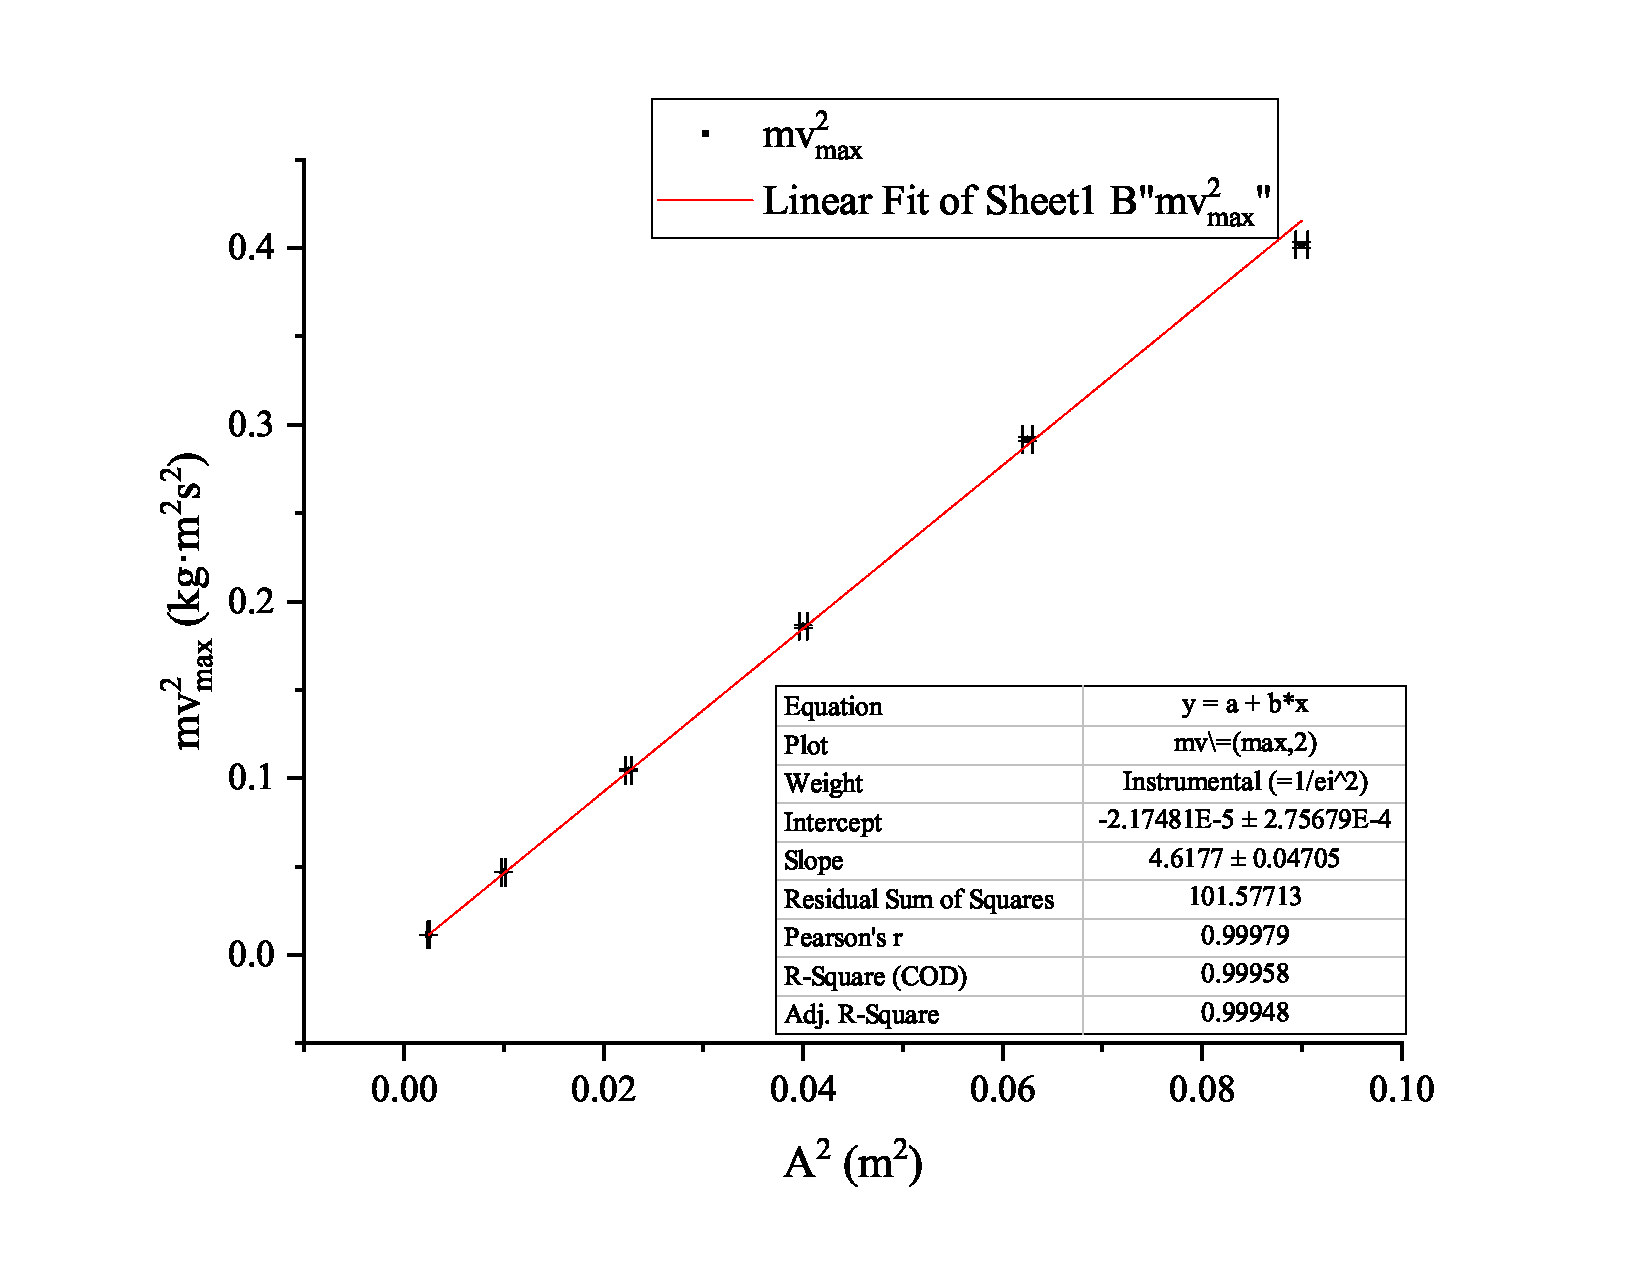
\includegraphics[width=1\linewidth]{12.eps}
		\caption{The linear fit of $v_{max}^2$ vs. $A^2$.}
	\end{figure}
	The linear fit of $M$ vs. $T^2$ is given by equation $M=\alpha T^2+\beta$. From the graph we know that the spring constant also the slope $\alpha=4.6177\ \rm{[kg\cdot m^2/s^2]}$, the intercept $\beta=-2.17481\times10^{-5}\ \rm{kg/s^2}$, the uncertainty of the slope $u_{k_M}=0.13\ \rm{kg/s^2}$. The Pearson's r is equal to 0.99979, very close to 1. Hence, we can deduce that $mv_{max}^2$ vs. $A^2$ has a linear relationship.
	\subsection{Mass Measurement Data}
	In the end of the exercise, we measure a set of masses that involve in calculation shown in Table 13. Note that
	\begin{equation*}
	M_0=m_{\rm{obj}}+\dfrac{1}{3}m_{\rm{spr1\&2}}
	\end{equation*}
	\begin{table}[H]
		\centering
		\begin{tabular}{|c|c|}
			\hline
			Measurement&$m$ [kg] $\pm$ 0.00001 [kg]\\
			\hline
			object with I-shape $m_{\rm{obj}}$&0.17457\\
			\hline
			object with U-shape $m_{\rm{obj}}$&0.17549\\
			\hline
			mass of springs 1 \& 2 $m_{\rm{spr1\&2}}$&0.0.2175\\
			\hline
			equivalent mass with I-shape $M_{0I}$&0.18182\\
			\hline
			equivalent mass with U-shape $M_{0U}$&0.18274\\
			\hline
		\end{tabular}
	\caption{Mass measurement data.}
	\end{table}
	\section{Conclusions and Discussion}
	In this experiment, we test the spring constants of two springs and their series. The results are
	\begin{equation*}
	k_1=(2.34\pm0.04)\ \rm{N/m}
	\end{equation*}
	\begin{equation*}
	k_2=(2.38\pm0.06)\ \rm{N/m}
	\end{equation*}
	\begin{equation*}
	k_{1,2}=(1.170\pm0.014)\ \rm{N/m}
	\end{equation*}
	Since the two springs are in series, we want to show that they satisfy the law of series of springs.
	\begin{equation*}
	k_s=\dfrac{k_1k_2}{k_1+k_2}=1.180\ \rm{N/m}
	\end{equation*}
	We check the relative error between $k_{1,2}$ and $k_s$ by $\dfrac{|k_{1,2}-k_s|}{k_s}$,
	\begin{equation*}
	error=\dfrac{\left|1.180-1.170\right|}{1.180}\times100\%=0.85\%
	\end{equation*}
	The relative error is small enough that the series is within the limit of Hooke's Law.
	
	When we want to show the linear relationship between $M$ and $T^2$, w e measure three spring constants $k_h$, $k_{I1}$, and $k_{I2}$. Using Eq. (4), the slope in the linear fit
	\begin{equation*}
	\alpha=\dfrac{k_1+k_2}{4\pi^2}=0.11956\ \rm{N/m}
	\end{equation*}
	Then the relative errors with different inclinations are
	\begin{equation*}
	error_{h}=\dfrac{|0.11826-0.11956|}{0.11956}\times100\%=13.6\%
	\end{equation*}
	\begin{equation*}
	error_{I1}=\dfrac{|0.11875-0.11956|}{0.11956}\times100\%=8.47\%
	\end{equation*}
	\begin{equation*}
	error_{I2}=\dfrac{|0.11880-0.11956|}{0.11956}\times100\%=7.95\%
	\end{equation*}
	These relative errors vary from the theorital values, so the support of the linear relationship between $M$ and $T^2$ need further explained. When adjusting the air track, the air flow blown from holes on the air track is  weaker than that on the other one, so there may be considerable friction. Besides, we find that all the three experimental values are lower than the theoretical value, which indicates tha the two springs are not attached as a series perfectly. For example, one end is attached on the rubber band fixed on one end of the air track forms an inclination from the horizontal plane.
	
	When we want to show that the period $T$ and the amplitude $A$ have no linear relationship. The Pearson's r turns out to be 0.88813 much smaller than 1 compared with moth linear fittings, so we can conclude that they are not related linearly.
	
	When we want to show the linera relationship between the square of the maximum speed $v_{max}^2$ and the amplitude $A$, by Eq. (6),
	\begin{equation*}
	\alpha=k_E=(4.62\pm0.13)\ \rm{kg/s^2}
	\end{equation*}
	Theoretically,
	\begin{equation*}
	k_t=k_1+k_2=4.72\ \rm{N/m}
	\end{equation*}
	Hence, the relative error is
	\begin{equation*}
	error=\dfrac{\left|4.72-4.62\right|{4.72}}\times100\%=2.12\%.
	\end{equation*}
	which is in a reasonable range but not very small, possibly due to the difference between the instantaneous speed and the average speed passing through the photoelectric gate.
	
	In addition, when the amplitude is too large, the damping effect is very obvious, probably due to the dissipation inner the spring, even out of the limit of Hooke's Law. When installing the shutters on the air track, it is important to make sure that the photoelectric gate only detect one light block during a half period. The metal plate on the masses and ends of shutters can interfere the detection so that the displayed period is a half of the real period.
	
	To improve the accuracy of this experiment, I would like to suggest that change the way to screw the shutters and the light source on the to avoid slipping back and forth. Fixing these experimental equipment can reduce errors.
	\newpage
	\renewcommand\thesection{\Alph{section}}
	\setcounter{section}{0}
	\section{Measurement uncertainty analysis}
	\subsection{Uncertainty of period measurments}
	The period measurements are single measurements with type-B uncertainty of 0.0001 s for 10$T$. For one period, the uncertainty $u_T=0.000001$ s.
	\subsection{Uncertainty of measurements for the time interval}
	The measurements for the time interval $\Delta t$ are single measurements with type-B uncertainty of 0.00001 s. The uncertainty $u_{\Delta t}=0.00001$ s.
	\subsection{Uncertainty of distance measurements}
	The distance measurements are single measurements with type-B uncertainty of 0.0001 m. The uncertainty $u_L=0.0001$ m.
	\subsection{Uncertainty of measurements for the difference between the stretched position and the initial position}
	The uncertainty of the measurements for the difference between the stretched position and the initial position $\Delta l_i=L_i-L_0$ can be calculated from the uncertainty of the distance measurements $u_L$ that
	\begin{equation*}
	u_{\Delta l}=\sqrt{u_L^2+u_L^2}=0.00014\ \rm{m}
	\end{equation*}
	\subsection{Uncertainty of measurements of $\bm{x_{in}}$ and $\bm{x_{out}}$}
	We have the type-B uncertainties of $x_{in}$ and $x_{out}$ $\Delta_{B,in}=\Delta_{B,out}=2\times10^{-5}$ m. Then, the type-A uncertainties
	\begin{equation*}
	\Delta_{A,in}=\dfrac{t_{0.95}}{\sqrt{3}}\sigma_x=\dfrac{t_{0.95}}{\sqrt{3}}\sqrt{\dfrac{\sum_{i=1}^3(\bar{x}-x_i)^2}{3-1}}=2.135\times10^{-5}\rm{m}
	\end{equation*}
	\begin{equation*}
	\Delta_{A,out}=\dfrac{t_{0.95}}{\sqrt{3}}\sigma_x=\dfrac{t_{0.95}}{\sqrt{3}}\sqrt{\dfrac{\sum_{i=1}^3(\bar{x}-x_i)^2}{3-1}}=2.135\times10^{-5}\rm{m}
	\end{equation*}
	Since $u_{x}=\sqrt{\Delta_A^2+\Delta_B^2}$, we can calculate the uncertainty
	\begin{equation*}
	u_{x_{in}}=\sqrt{(2.135\times10^{-5})^2+(2\times10^{-5})^2}\ \rm{m}=2.925\times10^{-5}\ \rm{m}\approx{0.00003}\ \rm{m}
	\end{equation*}
	\begin{equation*}
	u_{x_{out}}=\sqrt{(2.135\times10^{-5})^2+(2\times10^{-5})^2}\ \rm{m}=2.925\times10^{-5}\ \rm{m}\approx{0.00003}\ \rm{m}
	\end{equation*}
	\subsection{Uncertainty of $\bm{mv_{max}^2}$}
	Since we have $u_{x_{in}}=u_{x_{out}}=0.00003$ m, the uncertainty of the distance $\Delta x$ is
	\begin{equation*}
	u_{\Delta x}=\dfrac{\sqrt{u_{x_{in}}^2+u_{x_{out}}^2}}{2}=0.00002\ \rm{m}
	\end{equation*}
	Since if $F=\frac{X}{Y}$ the uncertainty propagation $u_r=\sqrt{u_{rX}^2+u_{rY}^2}$,
	\begin{equation*}
	u_{v_{max}}=v_{max}\sqrt{\dfrac{u_{\Delta x}^2}{\Delta x^2}+\dfrac{u_{\Delta t}^2}{\Delta t^2}}
	\end{equation*}
	Hence, we can calculate the uncertainty of the maximum speed:
	\begin{table}[H]
		\centering
		\begin{tabular}{|c|c|c|}
			\hline
			Measurement&$\Delta t$ [s]$\pm0.00001$ [s]&$u_{v_{max}}$ [m/s]\\
			\hline
			1&0.03965&0.0005\\
			\hline
			2&0.01962&0.0010\\
			\hline
			3&0.01313&0.0015\\
			\hline
			4&0.00985&0.0020\\
			\hline
			5&0.00786&0.003\\
			\hline
			6&0.0067&0.003\\
			\hline
		\end{tabular}
	\end{table}
	Based on that, we can calculate the uncertainty of $mv_{max}^2$ by
	\begin{equation*}
	u_{mv_{max}^2}=mv_{max}^2\sqrt{\dfrac{u_m^2}{m^2}+\dfrac{(2v_{max}u_{v_{max}})^2}{(v_{max}^2)^2}}
	\end{equation*}
	We list the uncertainty using the formula above,
	\begin{table}[H]
		\centering
		\begin{tabular}{|c|c|c|c|}
			\hline
			Measurement&$v_{max}$ [m/s]&$u_{v_{max}}$ [m/s]&$u_{mv_{max}^2}\ [\rm{kg\cdot m^2/s^2}]$\\
			\hline
			1&0.251&0.0005&0.00005\\
			\hline
			2&0.508&0.0010&0.00019\\
			\hline
			3&0.759&0.0015&0.0004\\
			\hline
			4&1.011&0.002&0.0007\\
			\hline
			5&1.267&0.003&0.0012\\
			\hline
			6&1.487&0.003&0.0016\\
			\hline
		\end{tabular}
	\caption{The Uncertainty of $mv_{max}^2$.}
	\end{table}
	\subsection{Uncertainty of $\bm{T^2}$}
	By the uncertainty propagation formula, the uncertainty of $T^2$ is
	\begin{equation*}
	u_{T^2}=2Tu_T
	\end{equation*}
	where $u_T=0.00001$ s. Using the formula above, we calculate the uncertainties of $T^2$ for each $T$ measured in the experiment.
	\begin{table}[H]
		\centering
		\begin{tabular}{|c|c|c|c|c|c|}
			\hline
			\multicolumn{2}{|c|}{Horizontal}&\multicolumn{2}{|c|}{Inclination 1}&\multicolumn{2}{|c|}{Inclination 2}\\
			\hline
			$T$ [s] $\pm0.00001$ [s]&$u_{T^2} [\rm{s^2}]$&$T$ [s] $\pm0.00001$ [s]&$u_{T^2} [\rm{s^2}]$&$T$ [s] $\pm0.00001$ [s]&$u_{T^2} [\rm{s^2}]$\\
			\hline
			1.54808&0.00003&1.54938&0.00003&1.55149&0.00003\\
			\hline
			1.58810&0.00003&1.59055&0.00003&1.59017&0.00003\\
			\hline
			1.62672&0.00003&1.62825&0.00003&1.62986&0.00003\\
			\hline
			1.66766&0.00003&1.66761&0.00003&1.67012&0.00003\\
			\hline
			1.70710&0.00003&1.70893&0.00003&1.70974&0.00003\\
			\hline
			1.74890&0.00003&1.74972&0.00003&1.75083&0.00004\\
			\hline
		\end{tabular}
	\caption{The uncertainty of $T^2$ for different inclinations.}
	\end{table}
	\begin{table}[H]
		\centering
		\begin{tabular}{|c|c|c|}
			\hline
			Measurement&$T$ [s] $\pm0.00001$ [s]&$u_{T^2} [\rm{s^2}]$\\
			\hline
			1&1.22816&0.00002\\
			\hline
			2&1.22858&0.00002\\
			\hline
			3&1.22839&0.00002\\
			\hline
			4&1.22859&0.00002\\
			\hline
			5&1.22881&0.00002\\
			\hline
			6&1.22883&0.00002\\
			\hline
		\end{tabular}
	\caption{The uncertainty of $T^2$ for different amplitudes.}
	\end{table}
	\subsection{Uncertainty of $\bm{A^2}$}
	Similar to the uncertainty of the square of the period, we have the uncertainty of the square of the amplitude
	\begin{equation*}
	u_{A^2}=2Au_A
	\end{equation*}
	where $u_A=0.001$ m, we calculate a set of uncertainties of $A^2$ in section 4.4 in Table 17.
	\begin{table}[H]
		\centering
		\begin{tabular}{|c|c|c|}
			\hline
			Measurement&$A$ [m] $\pm$ 0.001 [m]&$u_A^2$ [$\rm{m^2}$]\\
			\hline
			1&0.050&0.0001\\
			\hline
			2&0.100&0.0002\\
			\hline
			3&0.150&0.0003\\
			\hline
			4&0.200&0.0004\\
			\hline
			5&0.250&0.0005\\
			\hline
			6&0.300&0.0006\\
			\hline
		\end{tabular}
	\end{table}
	\subsection{Uncertainty of the slope of the linear fit of $\bm{mg}$ vs. $\bm{\Delta l}$}
	The uncertainty of the slope of the linear fit of $mg$ vs. $\Delta l$ is equal to the CI Half-Width.
	
	For spring 1,
	\begin{equation*}
	u_{k1}=0.04\ \rm{N/m}
	\end{equation*}
	with relative uncertainty
	\begin{equation*}
	u_{k1,r}=\dfrac{u_{k1}}{k_1}=1.7\%.
	\end{equation*}
	For spring 2,
	\begin{equation*}
	u_{k2}=0.06\ \rm{N/m}
	\end{equation*}
	with relative uncertainty
	\begin{equation*}
	u_{k2,r}=\dfrac{u_{k2}}{k_2}\times100\%=3\%.
	\end{equation*}
	For a series of spring 1 and spring 2,
	\begin{equation*}
	u_{k3}=0.014\ \rm{N/m}
	\end{equation*}
	with relative uncertainty
	\begin{equation*}
	u_{k3,r}=\dfrac{u_{k3}}{k_{1,2}}\times100\%=1.2\%.
	\end{equation*}
	\subsection{Uncertainty of the slope of the linear fit of $\bm{M}$ vs. $\bm{T^2}$}
	The uncertainty of the slope of the linear fit of $M$ vs. $T^2$ is equal to the CI Half-Width.
	
	For horizontal motion,
	\begin{equation*}
	u_{k1}=0.002\ \rm{N/m}
	\end{equation*}
	with relative uncertainty
	\begin{equation*}
	u_{k4,r}=\dfrac{u_{k4}}{k_4}=1.7\%.
	\end{equation*}
	For Inclination 1,
	\begin{equation*}
	u_{k5}=0.002\ \rm{N/m}
	\end{equation*}
	with relative uncertainty
	\begin{equation*}
	u_{k5,r}=\dfrac{u_{k5}}{k_5}\times100\%=1.7\%.
	\end{equation*}
	For Inclination 2,
	\begin{equation*}
	u_{k3}=0.001\ \rm{N/m}
	\end{equation*}
	with relative uncertainty
	\begin{equation*}
	u_{k6,r}=\dfrac{u_{k6}}{k_6}\times100\%=0.8\%.
	\end{equation*}
	\subsection{Uncertainty of the slope of the linear fit of $\bm{T}$ vs. $\bm{A}$}
	The uncertainty of the slope of the linear fit of $T$ vs. $A$ is equal to the CI Half-Width.
	\begin{equation*}
	u_{\alpha}=3\ \rm{s/m}
	\end{equation*}
	with relative uncertainty
	\begin{equation*}
	u_{\alpha,r}=\dfrac{u_{\alpha}}{\alpha}=72\%.
	\end{equation*}
	\subsection{Uncertainty of the slope of the linear fit of $\bm{mv_{max}^2}$ vs. $\bm{A^2}$}
	The uncertainty of the slope of the linear fit of $T$ vs. $A$ is equal to the CI Half-Width.
	\begin{equation*}
	u_{\alpha}=0.13\ \rm{s/m}
	\end{equation*}
	with relative uncertainty
	\begin{equation*}
	u_{\alpha,r}=\dfrac{u_{\alpha}}{\alpha}=2.8\%.
	\end{equation*}
	\newpage
	\section{Data Sheet}
	\begin{figure}[H]
		\centering
		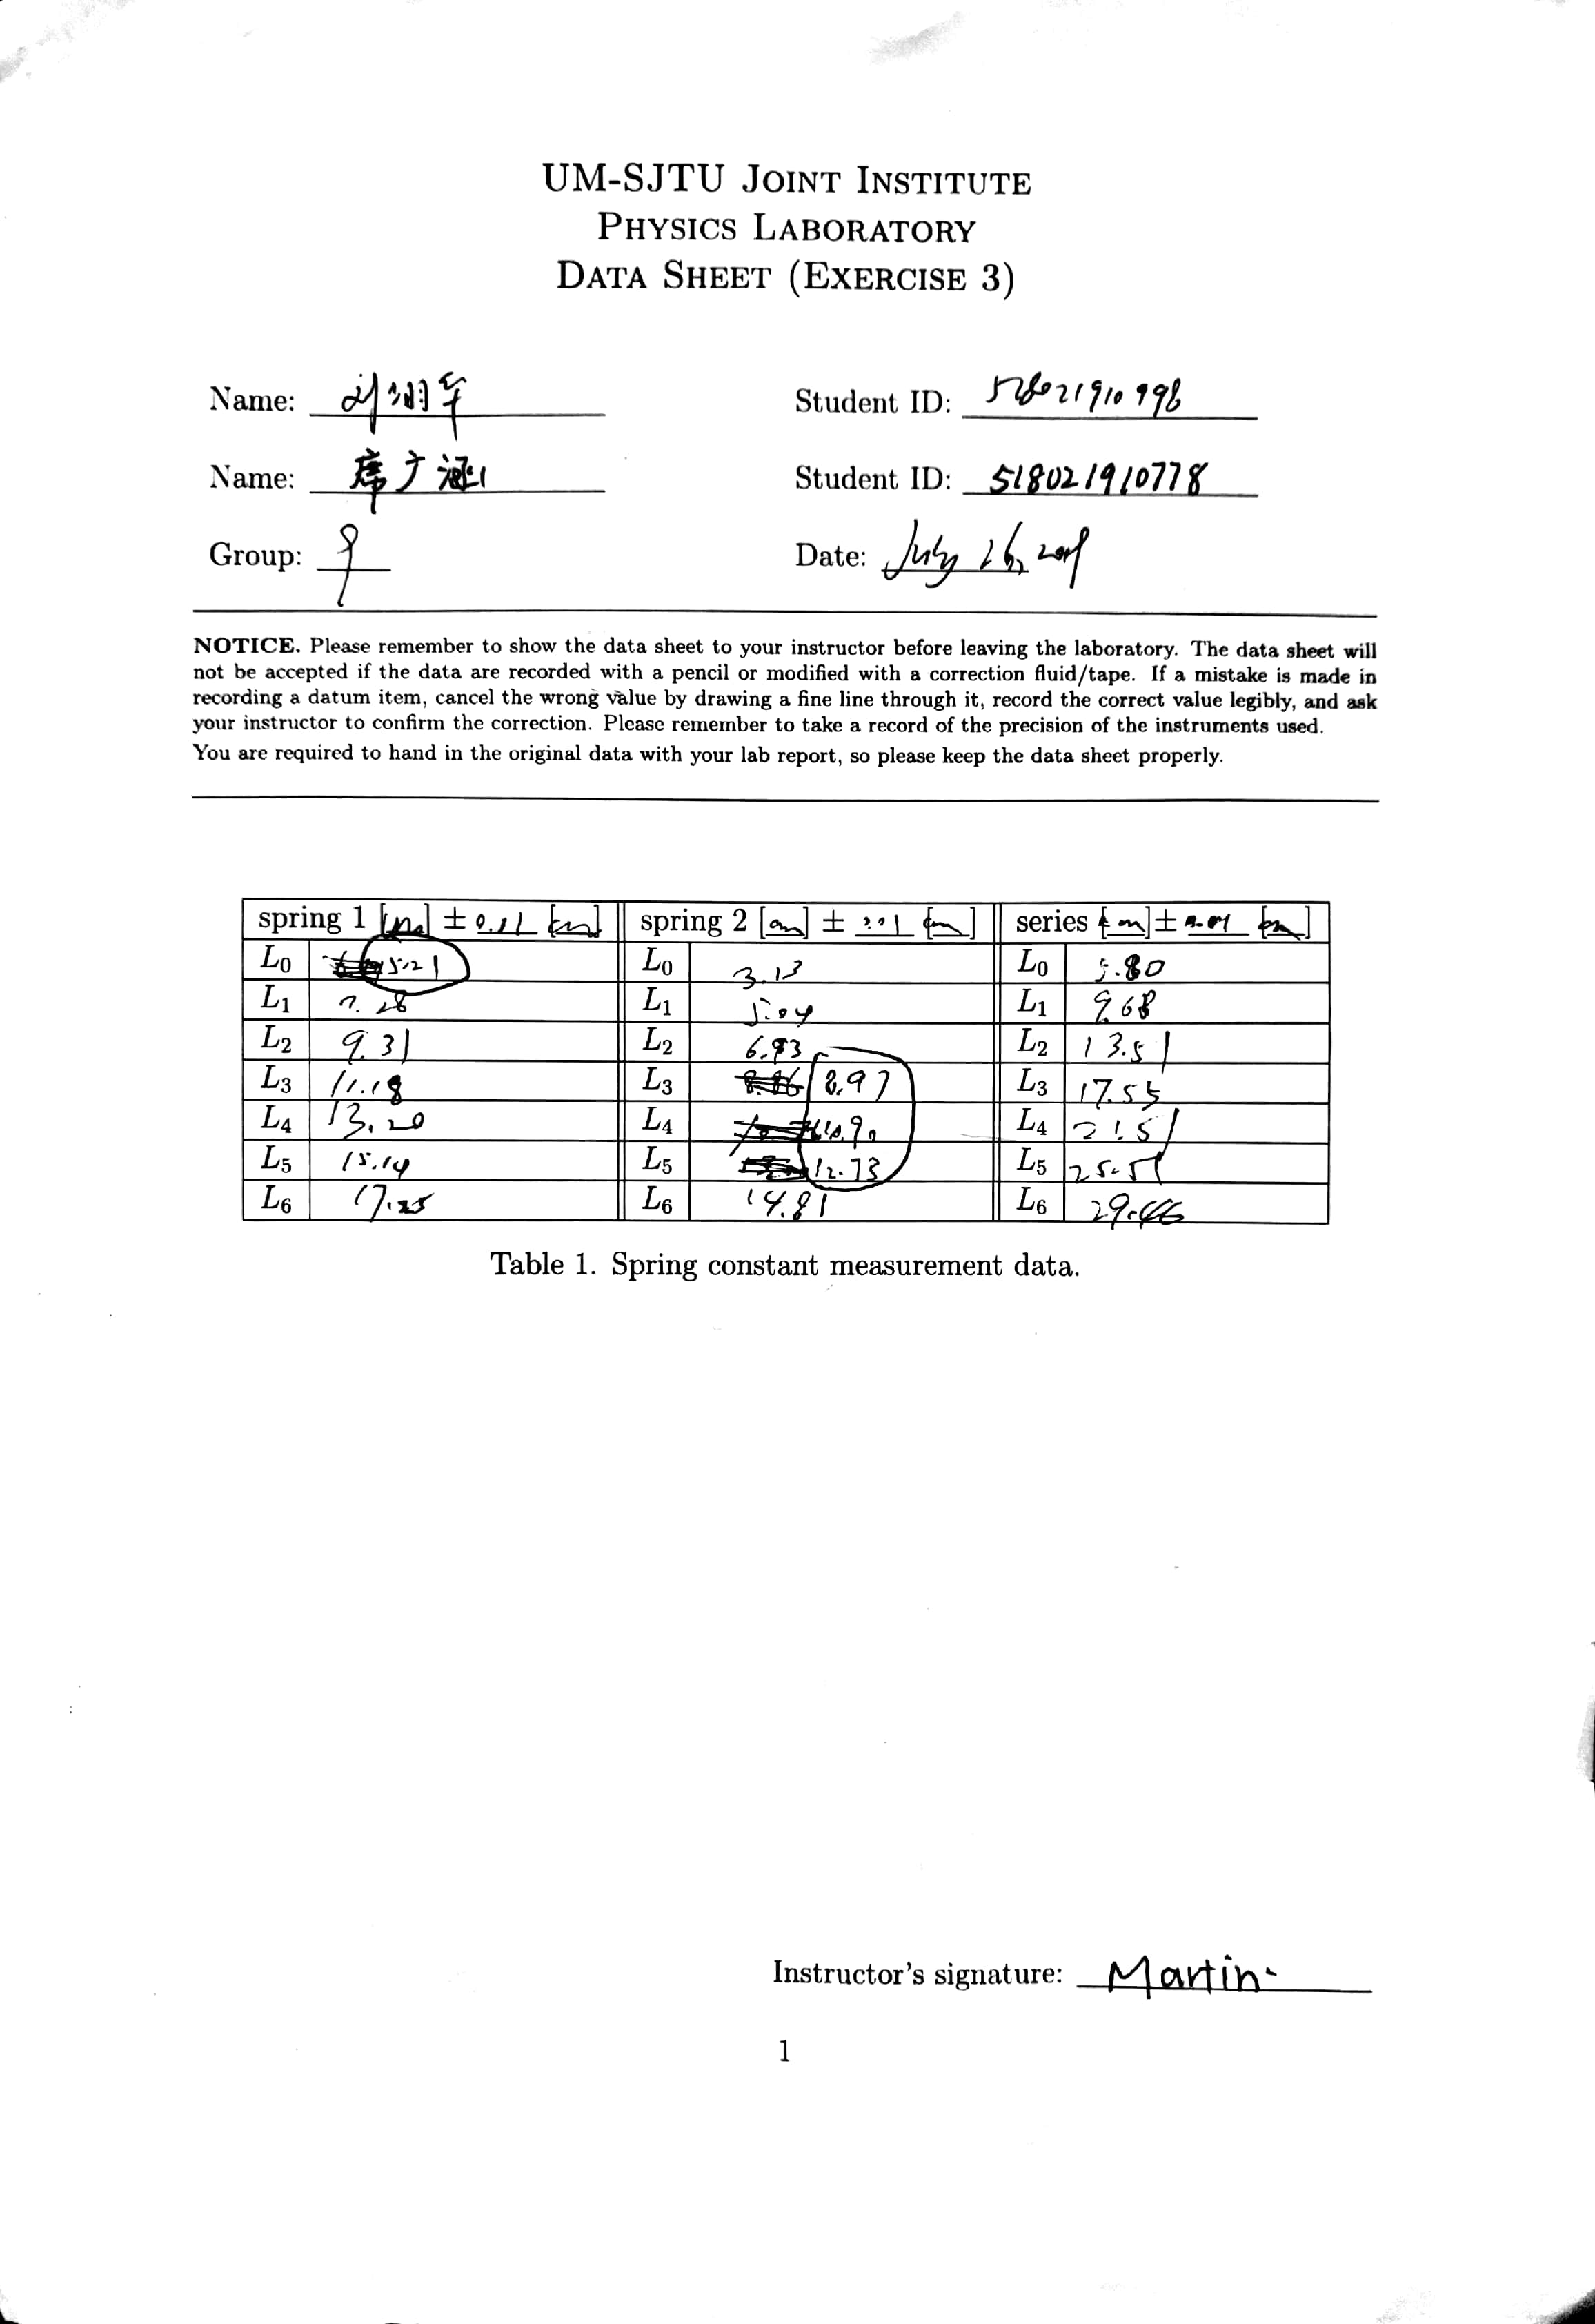
\includegraphics[width=1\linewidth]{13.jpg}
	\end{figure}
	\begin{figure}[H]
		\centering
		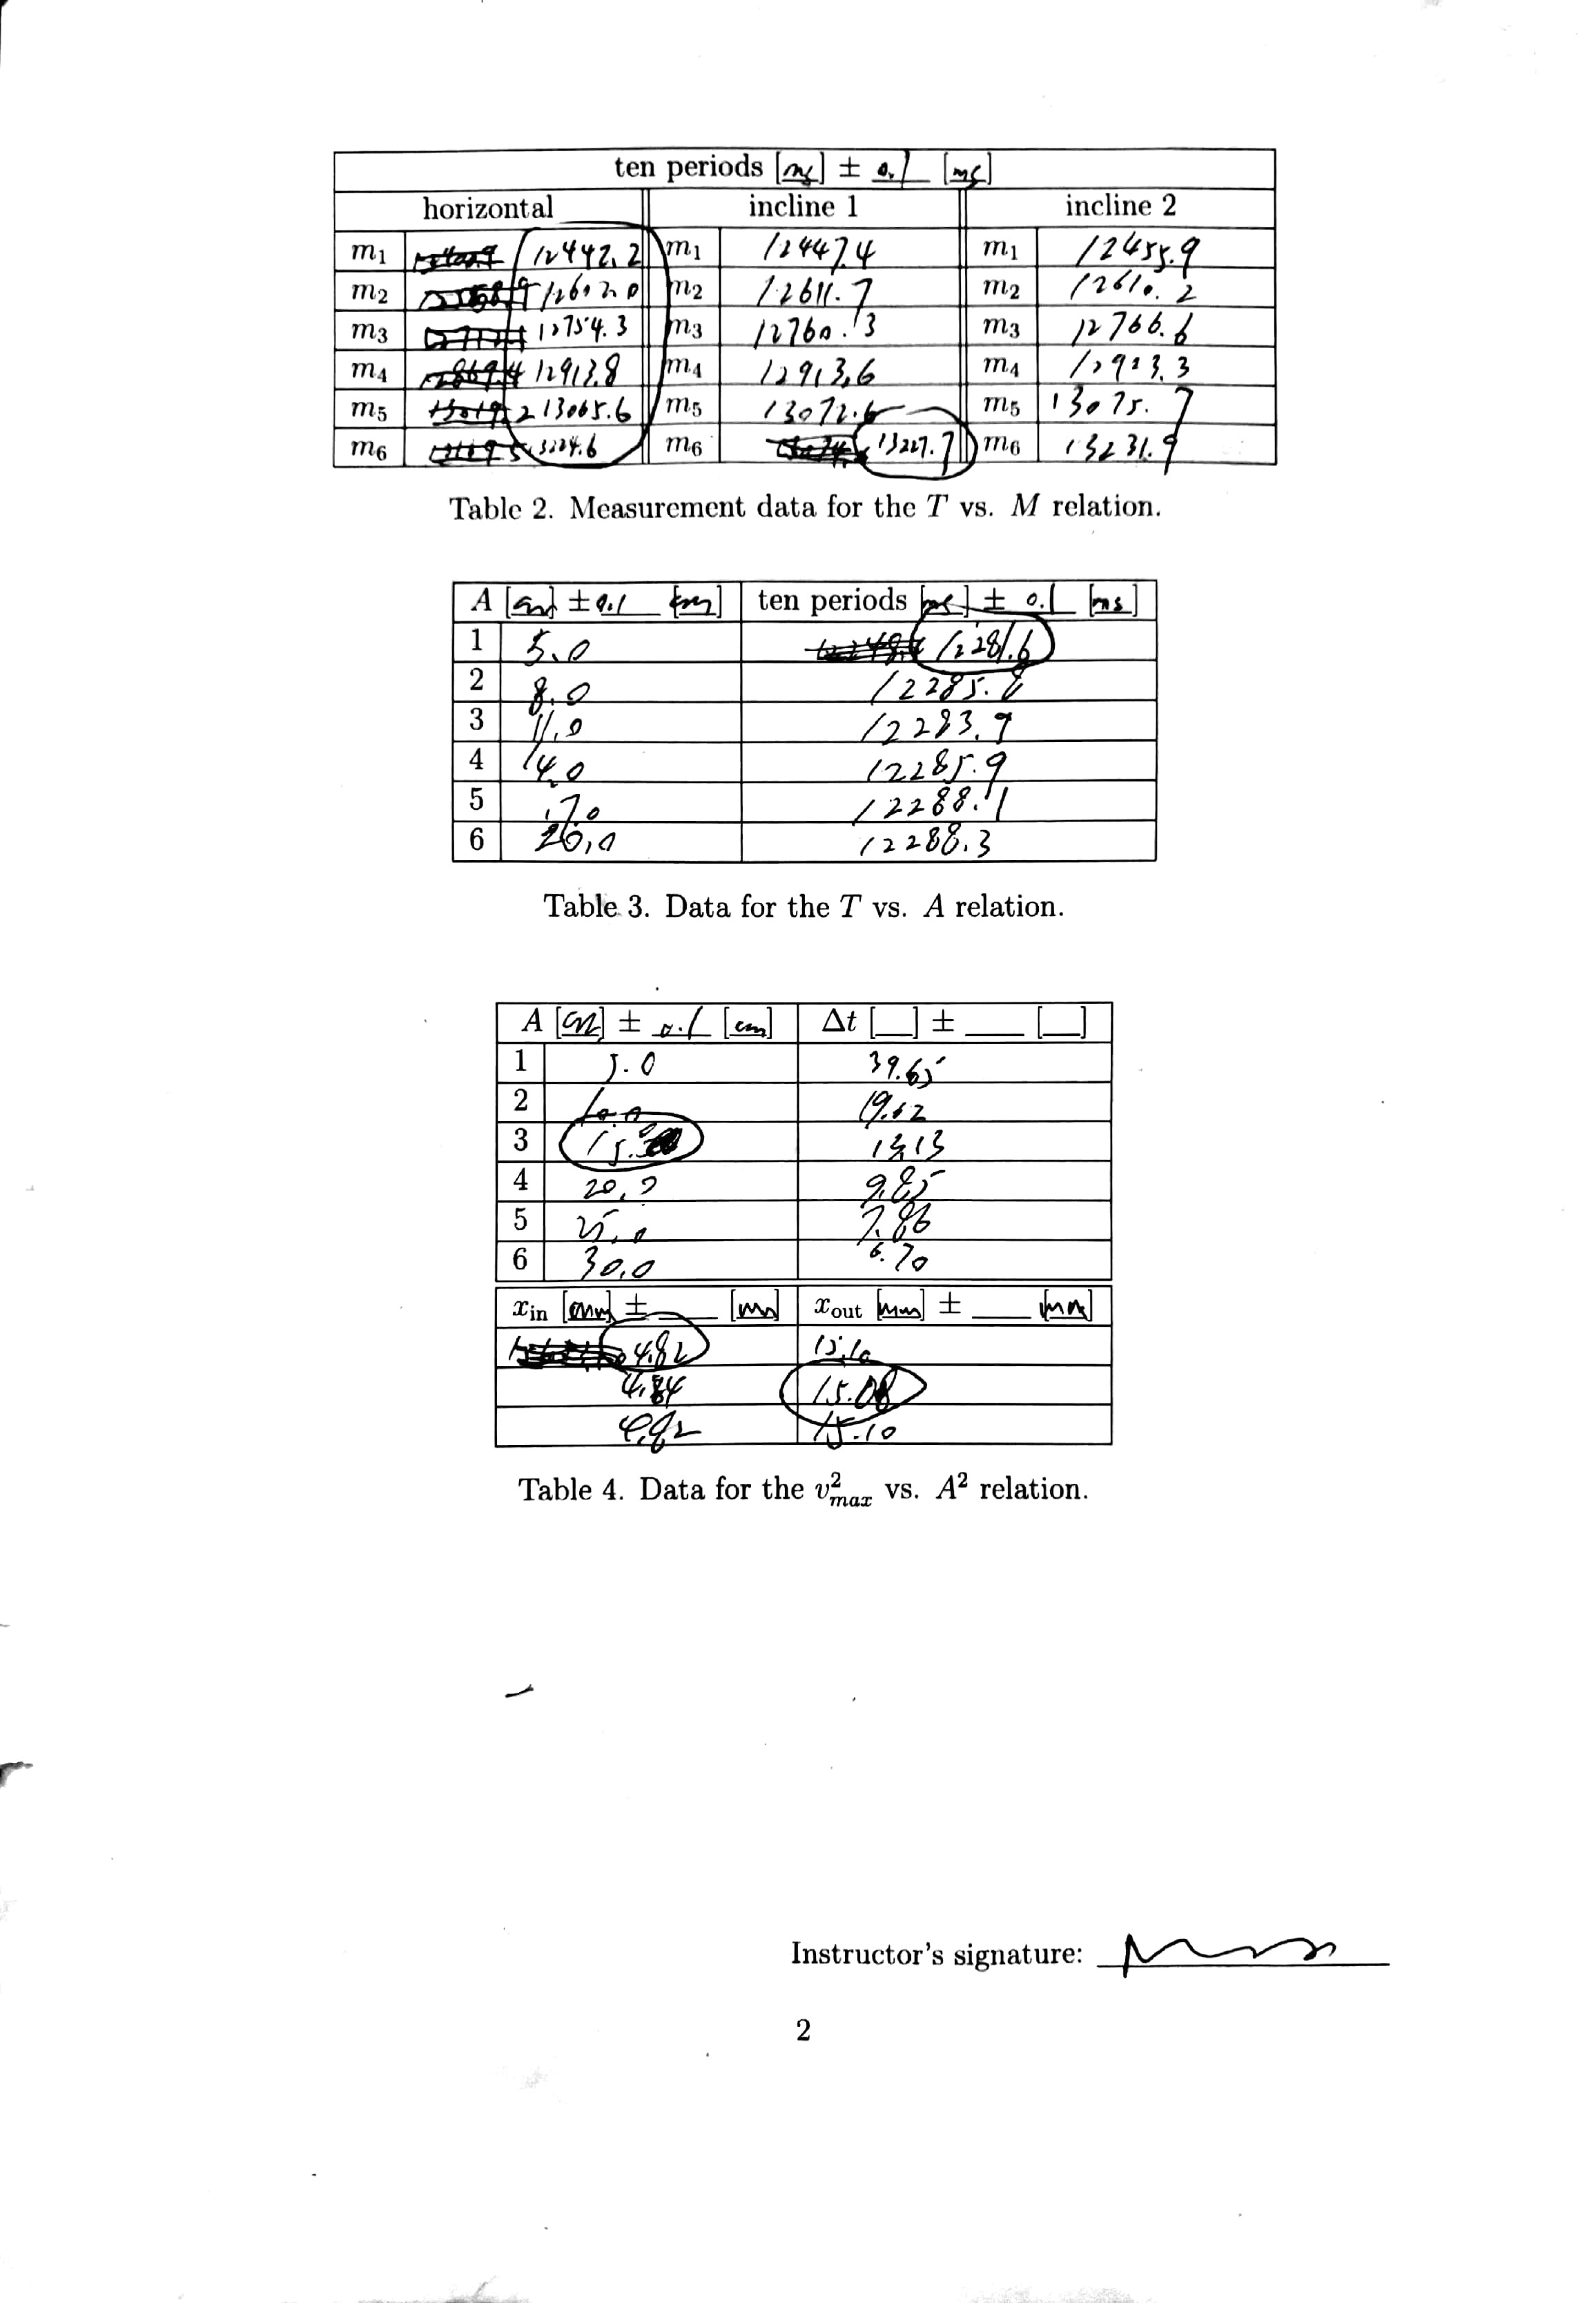
\includegraphics[width=1\linewidth]{14.jpg}
	\end{figure}
	\begin{figure}[H]
		\centering
		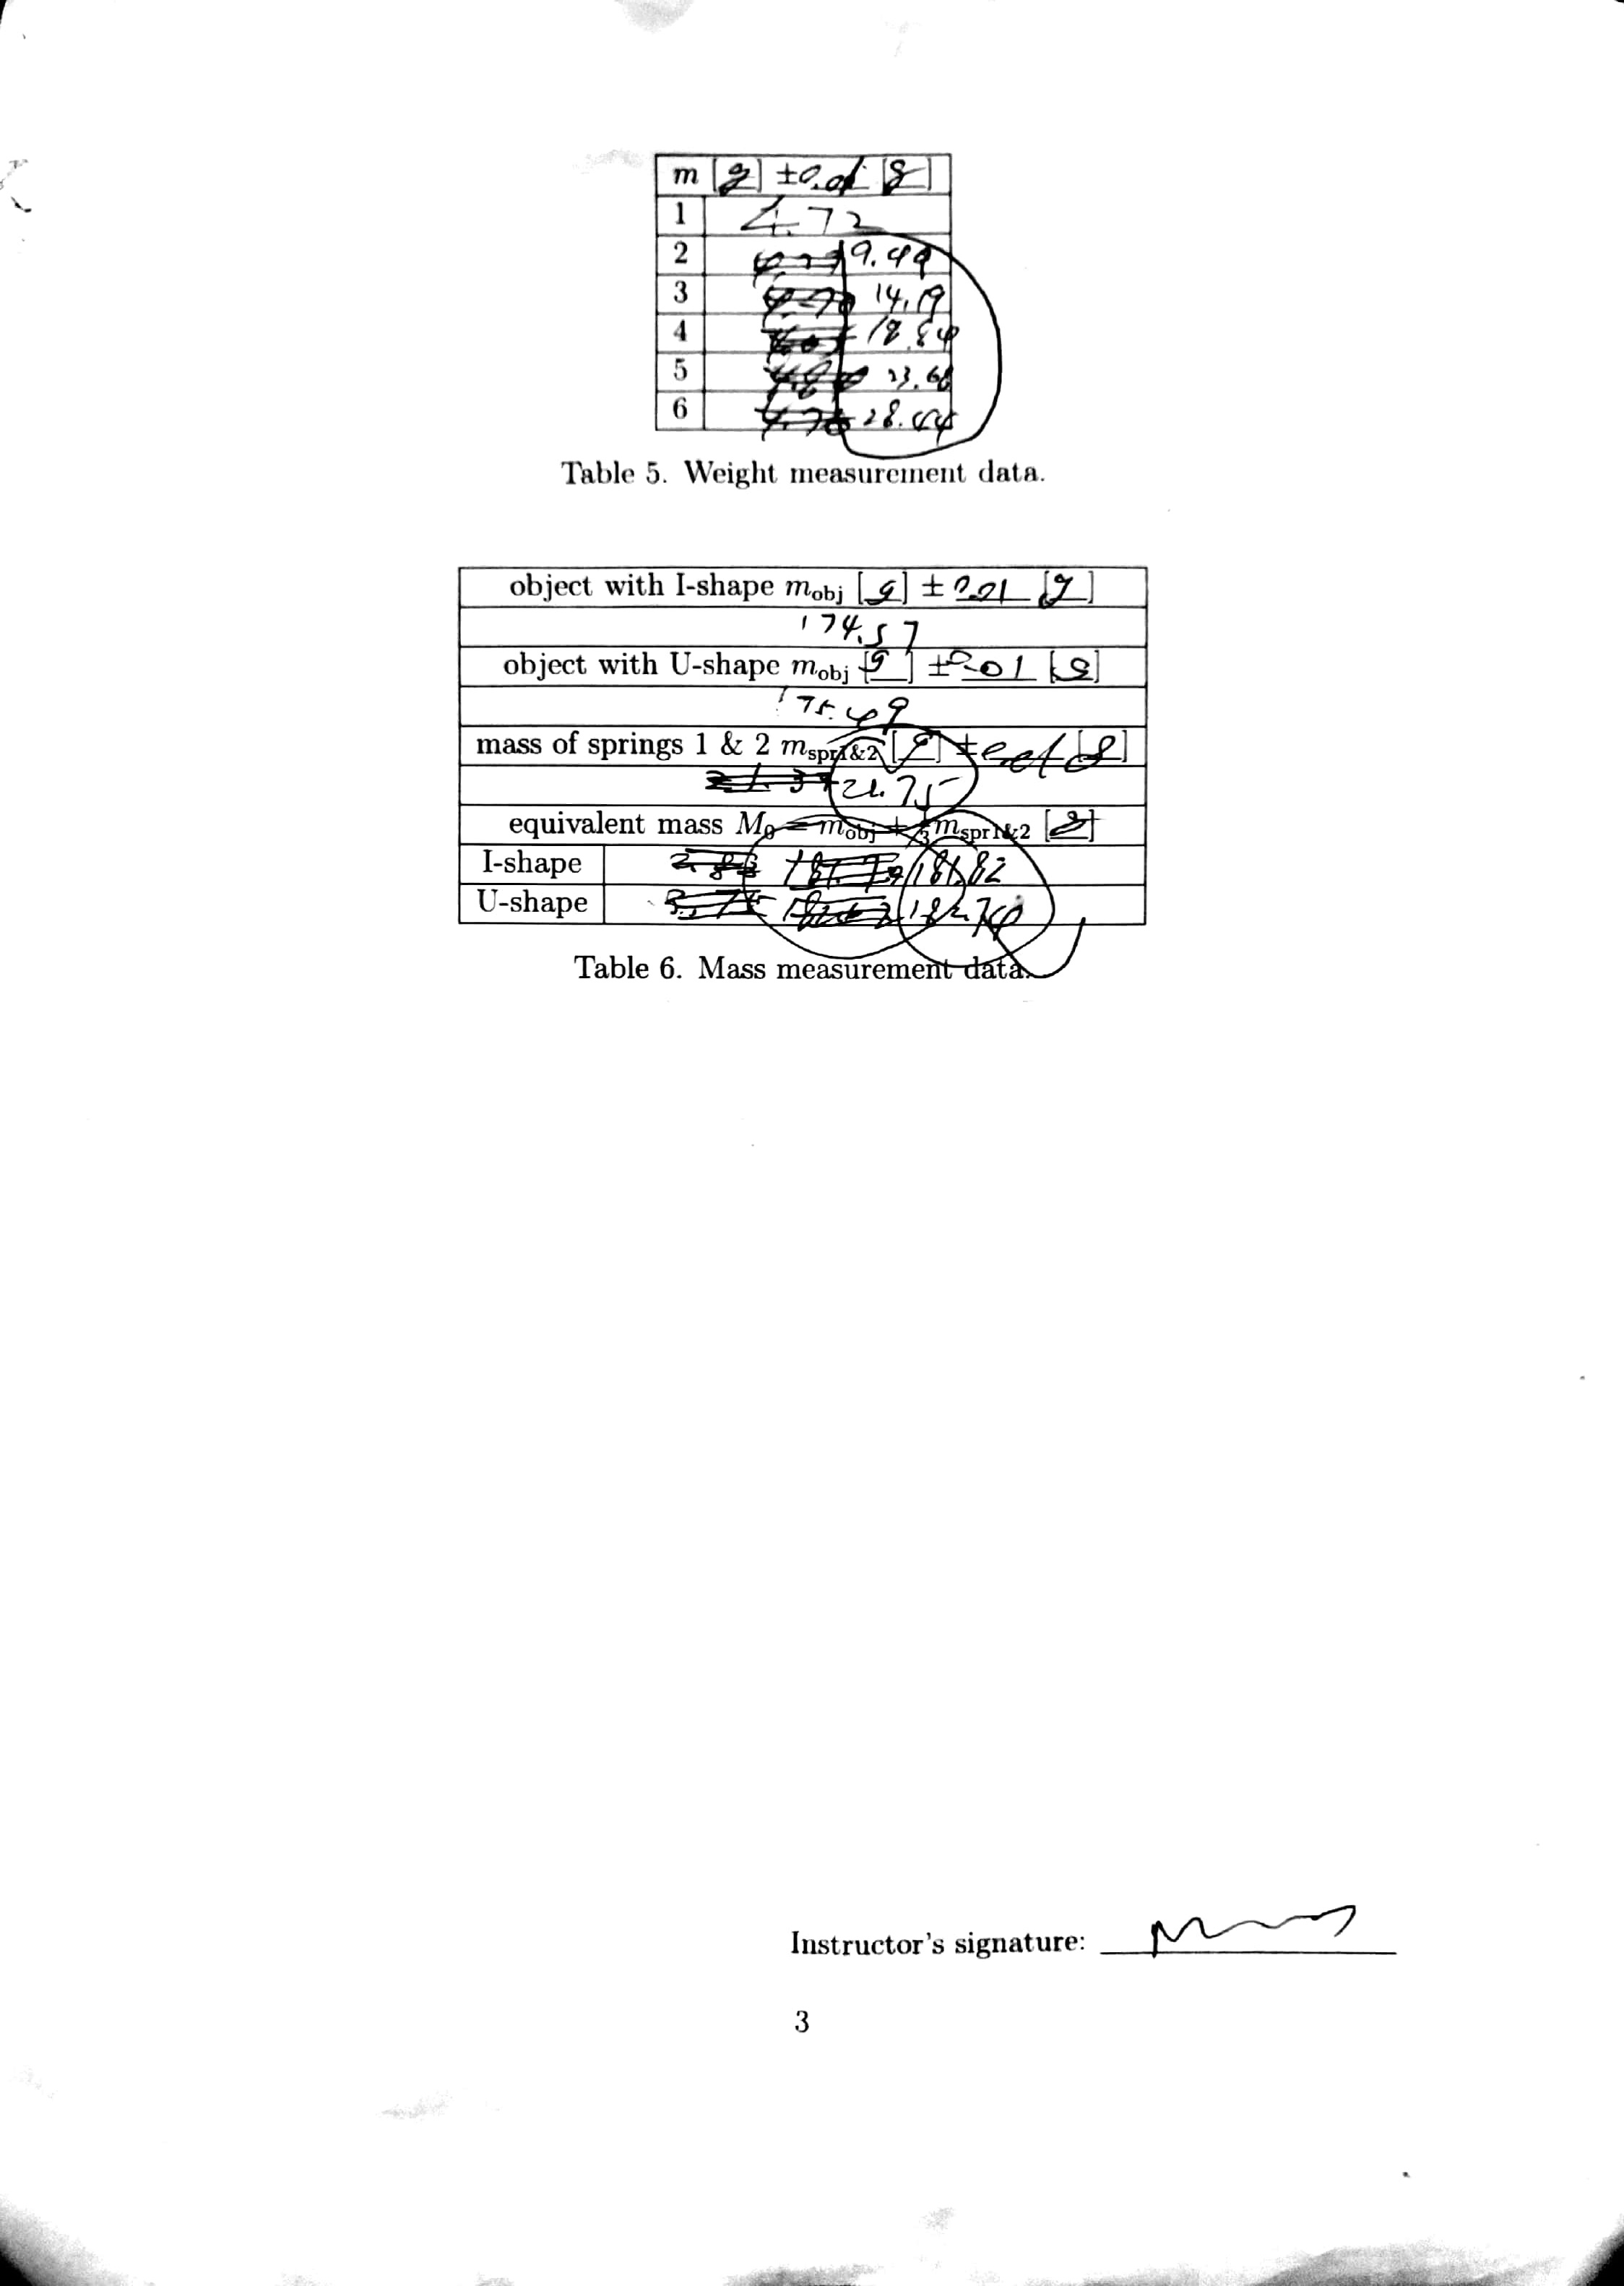
\includegraphics[width=1\linewidth]{15.jpg}
	\end{figure}
\end{document}